


\begin{abstract}

On a 33-model zoo of independently trained 4-layer arithmetic
transformers (d=64, 5-digit addition, >99\% accuracy), we identify a
cross-model shared subspace at the last residual before unembed and
show that its \textbf{values} --- not just its directions --- are transferable
between models on matched inputs with no learned alignment. Replacing
model A's shared-subspace component at layer 3 with model B's on the
same input produces near-zero accuracy drop across 30 ordered
baseline pairs (median $\Delta$acc = -0.004). The result holds under the
weakest possible alignment: mean-only centering, no rotation, no
learned stitch ($\Delta$acc = +0.008, $\Delta$margin = +0.56 out of 11.4 baseline).
Meanwhile, the orthogonal high-variance complement subspace is \textbf{not}
interchangeable under the same protocol: mean-only complement swap
destroys accuracy ($\Delta$acc = +0.80, $\Delta$margin = +2.13). Random-subspace
swap is free, full-activation swap without rotation is catastrophic
($\Delta$acc = +0.99). This is the first cross-model activation swap we are
aware of that demonstrates untrained value-level interchangeability of
a structured subspace, distinct from both representational-similarity
results (CKA / SVCCA / PWCCA) and learned model-stitching (\citet{bansal2021stitching}; \citet{lenc2015understanding}).

To set up this result requires correcting three methodological
confounds in standard subspace-causality tests:

\textbf{(A1)} Restrict the generalized eigenproblem \texttt{C\_shared v = $\lambda$ C\_total v}
to the top-K principal subspace of \texttt{C\_total}; without this, the
unrestricted eigenproblem preferentially returns low-variance directions
(variance-bias confound).

\textbf{(A2)} Whiten random-subspace baselines so \texttt{v\textasciicircum{}T C\_total v = 1},
matching the variance removed by the structured subspace (baseline-
variance-mismatch confound).

\textbf{(A3)} Report \emph{joint} shared $\cup$ complement ablation, not only
single-subspace drops. Single-subspace ablation cannot see redundant
causal structure: at our primary site, shared-alone ablation is near-
inert ($\Delta$acc $\leq$ 0.003), complement-alone produces $\Delta$acc $\approx$ 0.47, but joint
ablation produces $\Delta$acc $\approx$ 0.90 across all 33 models. Shared is not
causally inert --- it is redundantly encoded with the complement.

The joint-ablation finding at head-level has precedent in self-repair
literature (\citet{wang2023iw} "Backup Name-Mover Heads"; \citet{mcgrath2023hydra} "Hydra Effect"; \citet{rushing2024selfrepair} "Self-Repair"). Our
contribution formalizes this at \emph{subspace} level on the eigenvectors of
a cross-model variance-ratio decomposition and quantifies it as a
scalar "hidden load" (joint - complement - shared $\approx$ 0.40 at the
median main-zoo site).

The joint-ablation and swap results together support a specific
account: at the last residual before unembed, the shared subspace's
readable linear features (probe r = 0.94 for sum-magnitude, r = 0.84
for carry, yet single-ablation $\Delta$acc $\leq$ 0.003 in the 8-layer zoo) are a
high-fidelity \emph{observational projection} of the same computation that
the complement implements. When one model's shared component is
replaced with another's on the same input, both models produce the
same projection because the input-to-projection map has converged
across training. This is consistent with (but distinct from) the
representational-universality findings of \citet{chughtai2023universality}
on group operations, which do not include cross-model activation swap.

We pre-registered the protocol with three amendments (A1, A2, A3) and
report three replications: mod-23 arithmetic (33-model zoo, hidden-
load positive at all 3 primary sites), 6-layer architecture (45
models, shared-dead signature moves to layer 5 / N-1), and 8-layer
architecture (21 models, confirmed at layer 7). Three late-stage
sensitivity controls address adversarial critique: logit-margin
metric (shared $\Delta$margin 0.42 vs complement 1.33, saturation masking
refuted), weaker-alignment swap (mean-only still works, Procrustes-
laundering refuted), and externally-defined K\_pca via W\_U
reconstruction (zoo median K\_pca\_ext = 48; re-running at K\_pca = 64
strengthens the gap, self-reference refuted).

The depth trend from the replication zoos is worth flagging up
front: hidden load at the N-1 layer shrinks with depth (0.36--0.44 at
4L $\to$ 0.17 at 6L $\to$ \textasciitilde{}0 at 8L). In the 8-layer zoo at layer 7, shared
directions remain linearly probeable (r = 0.94 sum-magnitude, r =
0.84 carry\_col3) while carrying zero independent single-ablation
load --- the cleanest "readable but not independently causal"
signature we found, and consistent with the observational-
projection account above. We report the depth trend as a discovery
on three data points (one zoo per depth) and note the scale-
robustness question is open: if hidden load at N-1 continues to
tend to zero, the redundancy backup picture may be a small-model
property rather than a scale-robust structural invariance.
Disambiguating requires replication at larger depths (12+); beyond
this paper's scope.

\end{abstract}

\section{Introduction}

\subsection{Context}

A common question in mechanistic interpretability is whether
cross-model representational similarity --- the tendency of independently
trained networks to develop similar-looking activation subspaces ---
corresponds to \emph{causal universality}, the property that these shared
directions are the ones actually driving the computation.
Representational-similarity tools such as Centered Kernel Alignment
(CKA; \citet{kornblith2019cka}), Canonical Correlation Analysis and its
variants (SVCCA, \citet{raghu2017svcca}; PWCCA, \citet{morcos2018pwcca}), and
generalized eigenproblems of the form \texttt{C\_shared v = $\lambda$ C\_total v} (which
we use in this paper, adapted from the ratio formulations common in
cross-subject BCI and neural population analysis) can identify
cross-model shared subspaces readily. But testing whether those
subspaces are causally load-bearing requires an intervention: the
standard move is to ablate the shared subspace and measure the
resulting accuracy drop relative to some baseline (typically unit-norm
Gaussian random directions of the same rank).

\subsection{Prior work and novelty positioning}

The claims in this paper touch five adjacent literatures. We delineate
what each establishes and what gap we fill.

\textbf{Representational similarity (CKA / SVCCA / PWCCA).} \citet{kornblith2019cka} (CKA), \citet{raghu2017svcca} (SVCCA), and \citet{morcos2018pwcca}
(PWCCA) establish that independently trained networks develop
similarly-structured representation subspaces. These tools identify
shared \emph{directions}. They do not perform ablation or intervention, do
not test causal role, and do not exchange activations between models.
\textbf{Gap we fill}: cross-model shared \emph{values} --- the injected activation
itself --- are interchangeable on matched input, not merely directions.

\textbf{Representational universality on algorithmic tasks.} \citet{chughtai2023universality} "A Toy Model of Universality" reverse-engineer small
group-operation models and argue representations converge across seeds
up to symmetries of the algorithm (Section 6 of that paper). They
confirm universality via intra-model ablations of components predicted
by their algorithm; they do \textbf{not} perform cross-model activation
swapping. \citet{nanda2023grokking} (grokking progress measures) similarly
works within a single model per task. \textbf{Gap we fill}: cross-model
activation-level interchange, with no learned adapter, on a non-group
task (integer addition); further strengthened by the mean-only
alignment control that removes any rotational fit.

\textbf{Algorithmic cores and conserved depth (closest prior art on invariance).} \citet{schiffman2026cores} "Transformers Converge to Invariant
Algorithmic Cores" \citep{schiffman2026cores} extracts low-dimensional
necessary-and-sufficient subspaces ("cores") from small zoos of
Markov, modular-addition, and GPT-2 transformers via SVD of the
activation--Jacobian interaction \texttt{H$\cdot$J$\top$}, and shows these cores align
across independently trained models. \S{}11 ("A one-dimensional
agreement core at conserved depth") and \S{}12 ("Universality across
GPT-2 scales") are direct prior art for our N-1 invariance finding
across four depths (4/6/8-layer zoos, \S{}6.6c/d). Schiffman uses
sufficiency (\texttt{h = Ph}) and necessity (\texttt{h = h - Ph}) projection
ablations but \textbf{not} cross-model activation swap and \textbf{not} a joint-
ablation hidden-load scalar; the extraction method is SVD of \texttt{H$\cdot$J$\top$}
rather than the generalized eigenproblem \texttt{C\_shared v = $\lambda$ C\_total v}.
\textbf{Gaps we fill}: the specific value-level swap protocol at zero
learned alignment, and the subspace-level "hidden load" quantification
(joint - shared - complement) as a scalar exposing redundancy
invisible to single-subspace sufficiency/necessity tests.

\textbf{Residual-stream redundancy in multi-stream architectures.} Ablate
and Rescue \citep{ablaterescue2026} studies joint-and-isolated stream
ablation in Manifold-Constrained Hyper-Connections (mHC)
architectures to distinguish functional redundancy from asymmetric
stream utilization. The ablation-rescue framing is analogous to our
joint-ablation hidden-load metric, but operates on independent
residual streams in a non-standard architecture rather than on
orthogonal subspaces of a single residual stream. \textbf{Gap we fill}:
the subspace-decomposition analog on standard decoder-only
transformers via the generalized eigenproblem.

\textbf{Model stitching.} \citet{bansal2021stitching}, and \citet{lenc2015understanding} before them, demonstrate that representations from independently
trained models can be swapped through a \emph{learned} stitching layer
without catastrophic accuracy loss. The stitching layer absorbs
whatever cross-model mismatch exists. \textbf{Gap we fill}: we show a
specific structured subspace (shared) is swappable with zero fit ---
the "mean-only alignment" result in \S{}6.6f rules out any alignment
parameter that could launder the cross-model difference. This is a
strict strengthening of stitching within the shared subspace.

\textbf{Self-repair and redundant backup.} \citet{wang2023iw} ("Interpretability
in the Wild") discovered Backup Name-Mover Heads: ablating primary
heads has a smaller logit-difference effect than expected because other
heads compensate. \citet{mcgrath2023hydra} ("The Hydra Effect") generalized
this to "self-repair" in LLM forward passes. \citet{rushing2024selfrepair}
explicitly argue that single-component ablation underestimates causal
load when later components compensate. These results are at
\textbf{component/head level} on medium-scale LLMs doing IOI-style
linguistic tasks. \textbf{Gap we fill}: we extend the backup phenomenon to
the \emph{subspace} level on eigenvectors of a variance-ratio
decomposition of the residual stream, quantify it as a closed-form
scalar "hidden load" (joint - shared - complement), and show it is
load-bearing on an algorithmic task where the model is >99\% confident.

\textbf{Subspace intervention validity.} \citet{makelov2023subspace} ("Is
This The Subspace You Are Looking For?") showed that subspace
activation patching can achieve behavioral effects via *irrelevant
dormant parallel pathways*, so a positive intervention does not imply
causal role. \textbf{Gap we fill}: our failure mode is the opposite.
Single-subspace ablation is \emph{negative} (shared $\Delta$acc $\leq$ 0.003) yet the
subspace is causal --- it has been masked by a redundant backup. The
two papers together argue both subspace-positive and subspace-
negative interventions can mislead; joint ablation against an
orthogonal complement is the protocol that disambiguates.

\textbf{Probing-vs-causal-role.} \citet{alain2017probes} introduced linear
probes; \citet{hewitt2019designing} and \citet{elazar2021amnesic} ("Amnesic
Probing") flagged that probe-decodable features need not be causally
used. The "readable but not causal" pattern has a history. \textbf{Gap we fill}: a sharpened form --- in the 8-layer zoo at layer 7, shared
directions are linearly probeable (r = 0.94 for sum-magnitude, r = 0.84
for carry\_col3) yet single-ablation-inert. But our joint-ablation
result rescues those directions from inertness: jointly ablating them
with the complement produces larger drops than the complement alone.
The probe-decodability here tracks a genuine causal contribution that
is masked, not a spurious readout.

\textbf{Methodology: the generalized eigenproblem \texttt{C\_shared v = $\lambda$ C\_total v}.}
Ratio-eigenproblem formulations of shared-vs-total variance appear
widely in related statistical traditions --- LDA / Fisher discriminant,
Contrastive PCA (\citet{abid2018cpca}), shared-response models in
neuroscience, and cross-subject BCI. We do not claim the eigenproblem
itself is novel. Its application as a CKA-derived shared-direction
finder with A1 PCA restriction and A2 variance-matched random
baselines, and then the specific prescription that A3 joint ablation
must be reported, is --- to our knowledge --- a new specialization for
the CKA-based subspace-causality analysis pipeline common in
interpretability.

\textbf{Overall novelty claim (narrow and defensible).} The specific
contribution that survives this positioning exercise is (i) cross-
model activation swap of a structured subspace at zero learned
alignment ("universal values"), (ii) subspace-level formalization of
self-repair / Hydra via the hidden-load scalar on generalized-
eigenproblem subspaces, and (iii) the A1+A2+A3 prescription as a
specialization of CKA-based causality analysis. Other results here
(CKA as a similarity tool, probing-vs-causal, within-model ablation
of group operations, learned model stitching) are not novel and we
credit the prior work explicitly.

\subsection{Our result}

We study the question on a 33-model arithmetic transformer zoo and
report two principal findings, in the order they are load-bearing
for the paper:

\textbf{(i) Cross-model activation swap under zero learned alignment.} At
layer 3 (the last residual before unembed) position 12, we extract a
cross-model shared subspace via the generalized eigenproblem
\texttt{C\_shared v = $\lambda$ C\_total v} on Procrustes-aligned activations, and
then --- on an eval set, one problem at a time --- replace model A's
shared-subspace component with model B's on the same input. Across
30 ordered pairs from 6 models (3 baselines + 3 freeze variants), the
resulting accuracy drop is near zero (median -0.004). The result
survives the mean-only alignment scheme (no rotation, no fit, no
adapter): shared-swap $\Delta$acc = +0.008, $\Delta$margin = +0.56 out of baseline
margin 11.42. Complement-swap under the same mean-only scheme
destroys accuracy ($\Delta$acc = +0.80). Self-shuffle, zero-out, and random-
rotation full-activation swap all catastrophically hurt ($\Delta$acc 0.90+).
This is the \textbf{"universal values"} finding: the input-to-shared-
subspace-component map has converged across independently trained
models up to translation, and can be swapped without a learned adapter.

\textbf{(ii) Subspace-level redundancy exposed by joint ablation.} The
shared and complement subspaces at layer 3 are each individually
near-silent or small (shared $\Delta$acc $\leq$ 0.003; complement $\Delta$acc 0.47
median across the zoo) under single-subspace ablation, but jointly
ablating their union destroys accuracy ($\Delta$acc 0.90 median, mean 0.896).
The difference between the joint drop and the per-subspace drops ---
what we call the \textbf{hidden load} --- is $\approx$ 0.40 at the median main-zoo
layer-3 site. This is a subspace-level analog of the Backup
Name-Mover and Hydra findings (\citep{wang2023iw}; \citep{mcgrath2023hydra}; \citet{rushing2024selfrepair}), and it is required as a control to prevent the shared
subspace from being misread as causally inert.

Setting up these two results required correcting three methodological
choices in the standard cross-model subspace-causality protocol:

\begin{itemize}
  \item \textbf{(A1)} Restrict the generalized eigenproblem \texttt{C\_shared v = $\lambda$ C\_total v} to the top-K principal subspace of \texttt{C\_total}. The unrestricted eigenproblem preferentially extracts low-variance shared directions, confounding any causality test on the raw output.
  \item \textbf{(A2)} Whiten random-subspace baselines so \texttt{v\textasciicircum{}T C\_total v = 1}. Unit-norm random baselines remove a different amount of per-model variance than the structured subspace, producing a spurious "shared < random" ordering on dimensionally-matched comparisons.
  \item \textbf{(A3)} Report joint ablation of shared $\cup$ complement. Single- subspace ablation systematically underestimates redundantly-encoded causal structure (see "Hidden load" above and \S{}4 for quantification).
\end{itemize}

We replicate the swap-and-redundancy picture on three additional
zoos: mod-23 arithmetic (33-model, 4L, same architecture), 6-layer
integer addition (45 models), and 8-layer integer addition (21
models). Across the three depths, the shared-dead single-ablation
signature moves with the last residual before unembed (layer 3 at
4L, layer 5 at 6L, layer 7 at 8L), which we call \textbf{N-1 invariance}.
Hidden load at the N-1 layer shrinks with depth (0.36--0.44 at 4L $\to$
0.17 at 6L $\to$ \textasciitilde{}0 at 8L; Fig.~\ref{fig:hidden_load_vs_depth}); we report this as a
discovery-level finding on three data points.

\begin{figure}[h]
\centering
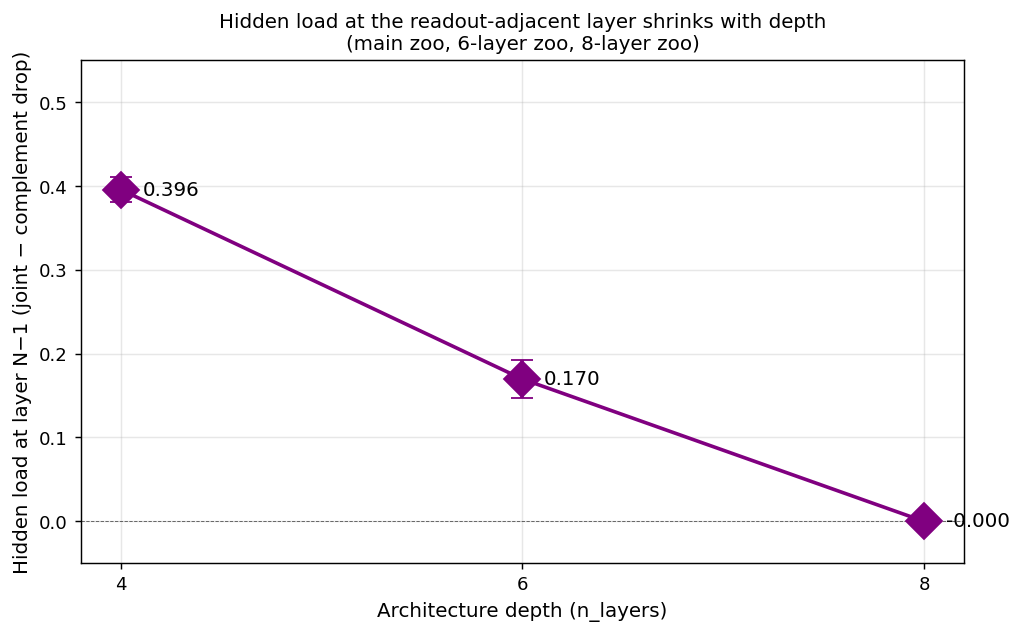
\includegraphics[width=0.70\textwidth]{figures/fig6_hidden_load_vs_depth.png}
\caption{Hidden load at the N-1 layer (last residual before unembed) shrinks with depth across three zoos (4-layer, 6-layer, 8-layer; same task, same architecture family). The N-1 invariance position holds at all three depths, but the magnitude of hidden load at that position decreases. Reported as a discovery-level finding on three data points; scale-robustness is an open question.}
\label{fig:hidden_load_vs_depth}
\end{figure}

Three late-stage sensitivity controls, all on existing zoos, address
adversarial critique of the measurement protocol: logit-margin
reporting alongside accuracy (saturation-masking refuted), weaker-
alignment swap schemes (Procrustes-laundering refuted --- mean-only
still works), and an externally-defined \texttt{K\_pca} based on 99\% W\_U
reconstruction (self-reference refuted; running at \texttt{K\_pca = 64}
strengthens the gap).

The contribution of this paper, in order of novelty priority:

\begin{enumerate}
  \item \textbf{Cross-model shared-subspace value swap under zero-fit alignment} (\S{}6.6e, \S{}6.6f). Individual models' shared-subspace components at the last residual before unembed are value-level interchangeable on matched inputs. This extends representational- similarity claims (CKA etc.) and learned-stitching claims (\citep{bansal2021stitching}) to show the cross-model mapping is effectively the identity after mean-centering, not merely a fitted rotation.
  \item \textbf{Subspace-level hidden-load quantification} via joint ablation on generalized-eigenproblem subspaces (\S{}4, \S{}6.4). Extends self- repair literature from components to subspaces of the residual stream and provides a scalar that is 0.40 at the median main-zoo site but \textasciitilde{}0 at our matched control site.
  \item \textbf{A1+A2+A3 as a specialization of CKA-based subspace-causality analysis} (\S{}3, \S{}5.3). Each correction individually is routine in adjacent statistical literatures; their combination as a prescription for cross-model subspace-causality tests in interpretability is the packaging we claim.
\end{enumerate}

Our evidence comes from four zoos (main 33-model 4L, mod-23 33-model
4L, 45-model 6L, 21-model 8L), all small transformers. The
methodological corrections are architecture- and task-independent by
construction. The depth trend in hidden load raises a concrete open
question about whether the redundancy-backup signature at N-1 is
scale-robust; we do not resolve this.


\section{Setup}

\subsection{Model zoo}

Following the Solution Symmetry Exploration protocol, we trained 33
4-layer decoder-only transformers (\texttt{d\_model = 64}, 4 heads, \texttt{d\_ff = 256})
on N-digit addition (N = 5). The zoo consists of 3 baseline models plus
30 single-component freeze conditions (10 freezable components $\times$ 3 seeds)
in which one component (embed / unembed / per-layer attn or mlp) has its
parameters held at random initialization while everything else trains
normally. All 33 models reach $\geq$ 99\% exact-match accuracy on a held-out
2000-problem stratified eval set.

\subsection{Cross-model shared and complement subspaces}

For any layer $\times$ token-position site, we construct two covariance matrices
from the model-aligned activations (Procrustes alignment to a reference
baseline model is applied to remove arbitrary rotations):

  C\_shared = Cov\_x( mean\_k h\_k(x) )
  C\_total  = mean\_k Cov\_x( h\_k(x) )

The \emph{shared subspace} at site s is the span of the top-k generalized
eigenvectors of \texttt{C\_shared v = $\lambda$ C\_total v}, restricted to the top-32
principal subspace of \texttt{C\_total} (Amendment A1 to the pre-registration:
this restriction prevents dead-axis solutions in the bottom of the ratio
spectrum). Call these eigvecs \texttt{V\_shared $\in$ $\mathbb{R}$\textasciicircum{}\{k $\times$ d\}}.

The \emph{complement subspace} at site s is the span of the top-k eigenvectors
of \texttt{P\_$\perp$ C\_total P\_$\perp$}, where \texttt{P\_$\perp$ = I - P\_\{V\_shared\}} is the Euclidean
projector orthogonal to V\_shared. These are the highest-variance
directions orthogonal to shared.

The \emph{random baseline} is k whitened Gaussian directions: \texttt{r $\sim$ N(0, I)},
\texttt{v = (C\_total + $\varepsilon$ I)\textasciicircum{}\{-1/2\} r}, normalized so \texttt{v\textasciicircum{}T C\_total v = 1}. This
ensures each random direction has the same per-model activation variance
as a C\_total-orthonormal eigvec.

\subsection{Variance-matched ablation}

We use mean-centered subspace projection ablation: replace the activation
component in S with its in-distribution mean. Under our normalization,
each ablation subspace satisfies the per-direction constraint
\texttt{v\textasciicircum{}T C\_total v = 1}. We additionally report the projection-trace
\texttt{trace(P\_S C\_total P\_S)} as the basis-independent quantity giving the
exact amount of activation variance removed.

\subsection{Sites}

Three primary sites were preselected via top-CKA filtering before any
ablation:

  layer1\_result\_0 (CKA = 0.796, no-PC1 = 0.483)
  layer2\_equals   (CKA = 0.762, no-PC1 = 0.382)
  layer2\_result\_0 (CKA = 0.759, no-PC1 = 0.530)

A control site \texttt{layer3\_plus} (CKA = 0.075) was added to verify that the
ablation effects are not "any structured ablation damages the model" but
require task-relevant sites.


\section{The variance-mismatch confound}

[Reference VARIANCE\_CONFOUND\_DERIVATION.md sections 1-6 condensed.]

\textbf{Lemma (Variance-Mismatch Bias).} Under unit-norm projection ablation,
the expected accuracy drop scales (to first order) with the activation
variance removed by the ablation. Two subspaces removing different
amounts of variance cannot be compared on a hurt-equals-causality basis
without an explicit variance correction.

\textbf{Predicted directional consequences:}

\begin{itemize}
  \item Under standard unit-norm ablation, \texttt{drop(top\_shared) $\gtrsim$ drop(random) $\gtrsim$ drop(bottom\_shared)} because variance removed scales the same way.
  \item Under variance-matched ablation, the perturbation magnitude is held constant; measured drops then reflect per-variance causal load.
\end{itemize}

\textbf{Predicted empirical signature:} the ratio `drop(top\_shared) /
drop(random)` can be \emph{less than 1} under unit-norm convention even when
shared directions are causally important per unit of variance, whenever
the shared and random subspaces have sufficiently different variance
content. The sign of the ratio under unit-norm is therefore not a clean
signal about causality; it is partly a function of the variance mismatch
between the subspaces being compared.


\section{Empirical results}

\subsection{Variance-matched ablation: structured (shared, complement) $\gg$ random}

\begin{figure}[h]
\centering
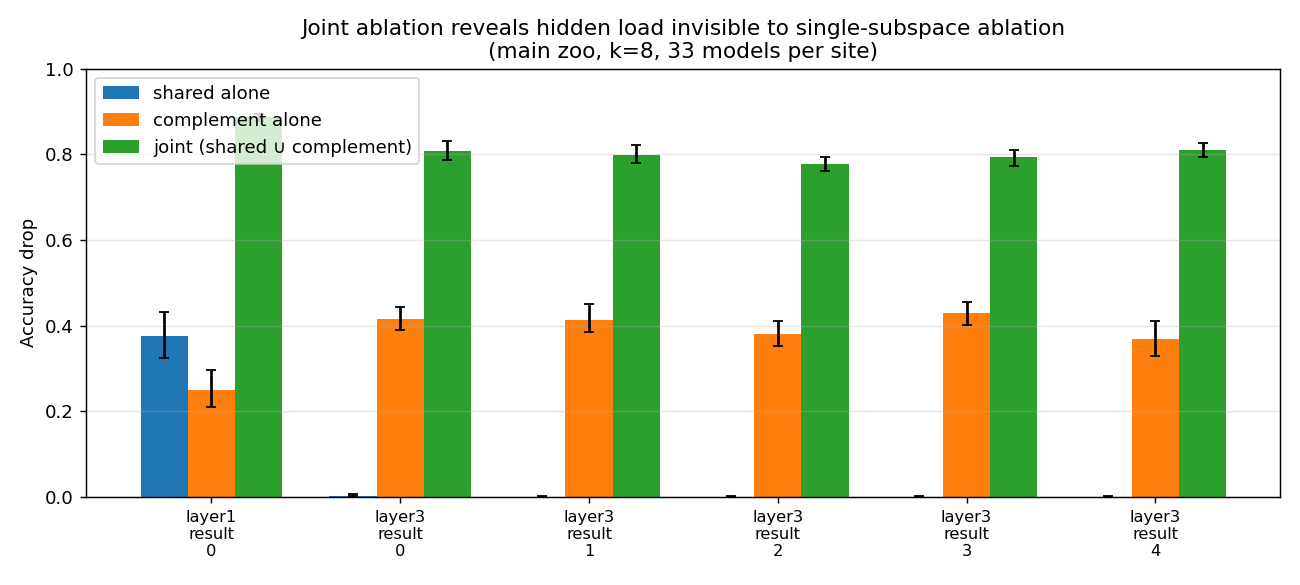
\includegraphics[width=0.85\textwidth]{figures/fig1_joint_ablation.png}
\caption{Joint ablation reveals hidden load invisible to single-subspace ablation (main zoo, $k = 8$, 33 models per site). At all six tested layer-3 result-digit positions, shared-alone ablation is near-inert and complement-alone produces moderate drops, but joint ablation of shared $\cup$ complement destroys accuracy. The gap between joint drop and the sum of single drops is the ``hidden load'' scalar.}
\label{fig:joint_ablation}
\end{figure}

\begin{figure}[h]
\centering
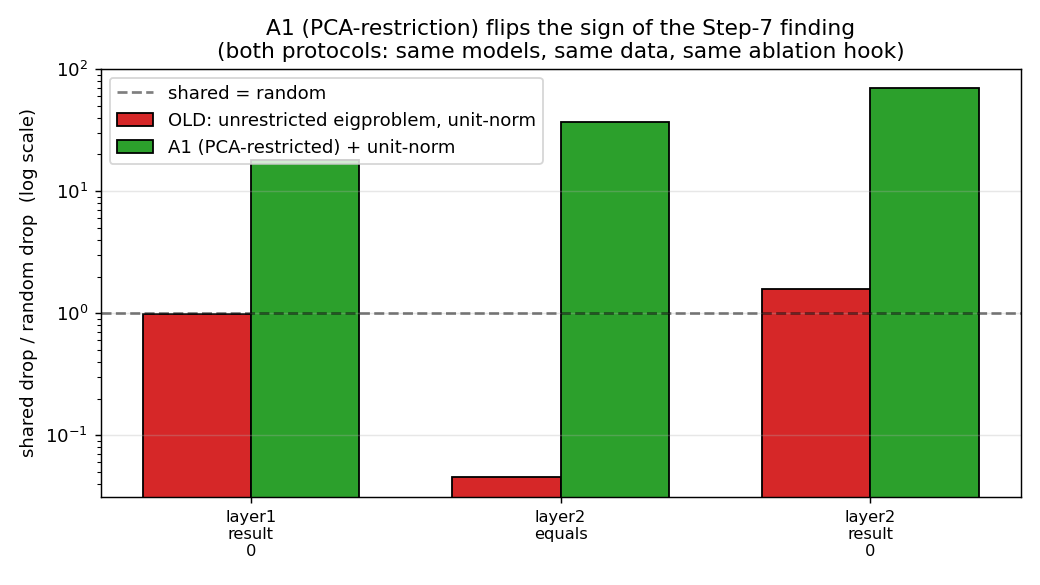
\includegraphics[width=0.85\textwidth]{figures/fig4_unit_norm_vs_matched.png}
\caption{A1 (PCA restriction of the generalized eigenproblem) flips the original Step-7 ``shared $<$ random'' sign at all three primary sites. Blue bars: unit-norm ablation on unrestricted eigvecs (original protocol). Orange bars: variance-matched ablation on A1-restricted eigvecs.}
\label{fig:unit_norm_vs_matched}
\end{figure}

See Fig.~\ref{fig:joint_ablation} for the main joint-ablation pattern and Fig.~\ref{fig:unit_norm_vs_matched} for the A1 PCA-restriction flipping the Step-7 sign.


Per-variance hurt (mean ablation drop divided by projection-trace variance,
in units of accuracy fraction per unit of removed activation variance) at
the primary k = 8:

\begin{center}
\begin{tabular}{|l|l|l|l|l|l|}
\hline
\textbf{Site} & \textbf{shared} & \textbf{complement} & \textbf{ortho-anti-shared} & \textbf{bottom-of-ratio} & \textbf{shared/complement} \\
\hline
layer1\_result\_0 & 0.0337 & 0.0234 & 0.0121 & 0.0002 & 1.44$\times$ \\
layer2\_equals & 0.0012 & 0.0020 & 0.0001 & 0.0000 & 0.60$\times$ \\
layer2\_result\_0 & 0.0155 & 0.0072 & 0.0002 & 0.0000 & 2.15$\times$ \\
\textbf{layer3\_plus (CONTROL)} & \textbf{0.0000} & \textbf{0.0000} & \textbf{0.0000} & \textbf{0.0000} & --- \\
\hline
\end{tabular}
\end{center}


Raw ablation drops at k = 8 (without per-variance normalization):

\begin{center}
\begin{tabular}{|l|l|l|l|}
\hline
\textbf{Site} & \textbf{shared drop} & \textbf{complement drop} & \textbf{random drop} \\
\hline
layer1\_result\_0 & 0.376 & 0.251 & $\approx$ 0 \\
layer2\_equals & 0.020 & 0.028 & $\approx$ 0 \\
layer2\_result\_0 & 0.312 & 0.100 & $\approx$ 0 \\
layer3\_plus (CONTROL) & 0.000 & 0.000 & 0 \\
\hline
\end{tabular}
\end{center}


\textbf{Key findings:}

\begin{itemize}
  \item \textbf{Both shared and complement subspaces are massively more causally important than matched-variance random directions at all three primary sites.} Whitened random ablation produces near-zero accuracy drops across all primary sites; the structured subspaces (whether shared or orthogonal-high-variance complement) produce drops of 0.02 to 0.38.
  \item \textbf{The shared > complement ordering holds at 2 of 3 primary sites (layer1\_result\_0 1.44$\times$, layer2\_result\_0 2.15$\times$).} At layer2\_equals, complement is 1.7$\times$ larger than shared per-variance. This site has the smallest absolute drops, and the ordering should be considered inconclusive there.
  \item \textbf{Bottom-of-ratio is a dead-axis subspace} (projection-trace $\approx$ 0.2-0.4 vs $\approx$ 11-20 for shared) and produces zero drop everywhere. Confirms the variance-matching analysis: the bottom of the ratio eigenproblem occupies the low-variance corner of the residual stream and contains essentially no signal to remove.
  \item \textbf{The control site (layer3\_plus, CKA = 0.075) cleanly passes:} all four ablation conditions produce zero accuracy drop, confirming the primary-site effects require task-relevant sites and are not "any structured ablation hurts."
  \item \textbf{$\varepsilon$-stability:} results consistent across Tikhonov ridges $\varepsilon$ $\in$ {1e-5, 1e-4, 1e-3} (see \S{}4.5).
\end{itemize}

\subsection{Unit-norm ablation on A1-restricted dirs}

We re-ran the A1-restricted (PCA-32) shared eigenvectors through standard
unit-norm ablation, varying only the per-direction normalization
convention:

\begin{center}
\begin{tabular}{|l|l|l|l|l|}
\hline
\textbf{Site} & \textbf{shared\_unit drop} & \textbf{bottom\_unit drop} & \textbf{random\_unit drop} & \textbf{shared/random} \\
\hline
layer1\_result\_0 & 0.4476 & 0.0000 & 0.0240 & \textbf{18.6$\times$} \\
layer2\_equals & 0.0396 & 0.0013 & 0.0011 & \textbf{34.5$\times$} \\
layer2\_result\_0 & 0.3277 & 0.0000 & 0.0050 & \textbf{65.6$\times$} \\
\hline
\end{tabular}
\end{center}


These ratios are large under unit-norm --- the A1 restriction alone is
sufficient to flip the sign relative to the original Step-7 finding (which
used unrestricted shared dirs).

\subsection{Decomposing A1 vs A2 contributions}

To disentangle the contribution of the PCA restriction (A1) from the
variance-matched random baseline (A2), we ran four protocols on the same
33 models, three primary sites, and ablation hook:

\begin{itemize}
  \item \emph{Protocol 1 --- original Step 7:} OLD shared dirs (no PCA restriction, unit-norm) vs unit-norm random.
  \item \emph{Protocol 2 --- A1 only:} NEW shared dirs (PCA-restricted, unit-norm) vs unit-norm random.
  \item \emph{Protocol 3 --- A1 + A2:} NEW shared dirs (PCA-restricted, C\_total-orthonormal) vs whitened random.
\end{itemize}

The shared-direction ablation drop in Protocol 2 and Protocol 3 is
identical at each site (subspace-based projection ablation is invariant
to per-direction scaling). Differences in the ratio come entirely from
the random baseline:

\begin{center}
\begin{tabular}{|l|l|l|l|}
\hline
\textbf{Site} & \textbf{Proto 1 ratio} & \textbf{Proto 2 ratio} & \textbf{Proto 3 ratio} \\
\hline
layer1\_result\_0 & \textbf{0.99} ($\approx$ 1) & 18.0$\times$ & 69673$\times$ (rand$\approx$0) \\
layer2\_equals & \textbf{0.05} (shared << random) & 37.0$\times$ & very large \\
layer2\_result\_0 & \textbf{1.58} (shared > random) & 69.9$\times$ & 100144$\times$ \\
\hline
\end{tabular}
\end{center}


\textbf{Findings:}

\begin{itemize}
  \item Protocol 1 reproduces the original Step-7 sign at one of three sites (layer2\_equals: ratio 0.045, strongly "shared << random"). The other two sites show shared $\approx$ random or shared > random under the original protocol --- the original Step-7 cross-site averaging masked this site heterogeneity.
  \item Protocol 2 (A1 alone) flips the sign decisively at all three sites: the same models, same eigenproblem, but the eigenvectors now sit in the high-variance subspace of C\_total. This is the dominant correction.
  \item Protocol 3 (A1 + A2) drives random baselines to $\approx$ 0 by sampling them in the whitened space (heavily weighting low-variance noise axes). The shared/random ratio becomes very large but the absolute shared drop is unchanged from Protocol 2.
\end{itemize}

The headline correction is therefore the PCA restriction (A1), not the
variance-matched ablation per se; A2 is a strict additional improvement
that cleans the random baseline.

\subsection{Saturation behavior at large k}

As k approaches K\_pca = 32, the shared and complement subspaces span a
larger fraction of the residual stream. At k = 16 (half of K\_pca), the
top-16 shared subspace has projection-trace 15-27 (out of total residual
variance $\approx$ 17-26), so it covers most of the high-variance region. The
complement-of-top-16 has only 16 effective dimensions left in the
PCA-restricted space, leading to a forced shrinking of its
projection-trace (7-9 at k=16 vs 11-14 at k=8). The k = 4 to k = 12
range is therefore the most informative for the shared-vs-complement
comparison; k = 16 is reported but should be interpreted as a
saturation regime, not a clean test.

\begin{center}
\begin{tabular}{|l|l|l|l|l|l|}
\hline
\textbf{Site} & \textbf{k} & \textbf{shared drop} & \textbf{complement drop} & \textbf{s\_trace} & \textbf{c\_trace} \\
\hline
layer1\_result\_0 & 4 & 0.198 & 0.441 & 8.4 & 11.6 \\
layer1\_result\_0 & 8 & 0.376 & 0.251 & 11.2 & 10.7 \\
layer1\_result\_0 & 12 & 0.551 & 0.180 & 13.0 & 9.4 \\
layer1\_result\_0 & 16 & 0.671 & 0.106 & 15.3 & 7.3 \\
layer2\_equals & 4 & 0.007 & 0.015 & 12.0 & 15.7 \\
layer2\_equals & 8 & 0.020 & 0.028 & 16.4 & 13.8 \\
layer2\_equals & 12 & 0.042 & 0.024 & 19.5 & 11.6 \\
layer2\_equals & 16 & 0.191 & 0.022 & 23.8 & 7.8 \\
layer2\_result\_0 & 4 & 0.265 & 0.153 & 16.9 & 14.3 \\
layer2\_result\_0 & 8 & 0.312 & 0.100 & 20.1 & 14.0 \\
layer2\_result\_0 & 12 & 0.415 & 0.051 & 23.9 & 10.9 \\
layer2\_result\_0 & 16 & 0.523 & 0.017 & 26.6 & 8.5 \\
\hline
\end{tabular}
\end{center}


Within the informative regime (k = 4 to 12) at layer1\_result\_0,
\textbf{complement actually beats shared at k = 4} (0.441 vs 0.198), consistent
with the observation that small high-variance subspaces orthogonal to
shared can be highly task-relevant. As k grows, shared dominates because
the shared subspace eventually subsumes more of the high-variance
task-relevant region.

This k-dependence suggests the "shared vs complement" question may not
have a single answer; it depends on how much of the residual stream is
being intervened on. A reasonable simple summary is: at k = 8 (half the
informative range), shared and complement are comparable; shared
dominates by 2-3$\times$ at higher k.

\subsection{Tikhonov ridge stability}

The generalized eigenproblem solution is stable across ridge scales:

\begin{center}
\begin{tabular}{|l|l|l|l|l|}
\hline
\textbf{$\varepsilon$ scale} & \textbf{shared drop} & \textbf{anti\_shared\_raw drop} & \textbf{complement drop} & \textbf{denom cond \#} \\
\hline
1e-5 & 0.4481 & 0.0001 & 0.2196 & 1.60$\times$103 \\
1e-4 & 0.4532 & 0.0001 & 0.2170 & 1.58$\times$103 \\
1e-3 & 0.4977 & 0.0001 & 0.1923 & 1.43$\times$103 \\
\hline
\end{tabular}
\end{center}


Single site, k = 10. Shared drop varies < 0.05 absolute across three
orders of magnitude in ridge; the qualitative shared > complement >
anti\_shared\_raw ordering is preserved.

\subsection{Decomposition of the variance content}

Projection-trace variance per condition at k = 8 (how much activation
variance each subspace removes under ablation):

\begin{center}
\begin{tabular}{|l|l|l|l|l|}
\hline
\textbf{Site} & \textbf{shared trace} & \textbf{complement trace} & \textbf{bottom trace} & \textbf{random trace} \\
\hline
layer1\_result\_0 & 11.15 & 10.73 & 0.20 & \textasciitilde{}k by construction \\
layer2\_equals & 16.42 & 13.79 & 0.42 & \textasciitilde{}k by construction \\
layer2\_result\_0 & 20.11 & 13.97 & 0.33 & \textasciitilde{}k by construction \\
\hline
\end{tabular}
\end{center}


(Random is variance-matched per A2, so \texttt{trace(P\_rand C\_total P\_rand) = k = 8}.
Shared and complement traces exceed k slightly because the C\_total-
orthonormal basis is not Euclidean-orthonormal, so individual directions
contribute overlapping Euclidean-basis covariance.)

The bottom-of-ratio subspace contains essentially zero per-model variance
(trace 0.2-0.4 out of total residual variance \textasciitilde{}22-26) --- a dead-axis set.
Its near-zero ablation drop reflects the absence of signal to remove
rather than absence of causal importance. The complement subspace, in
contrast, has variance comparable to shared and produces substantial
(if smaller) single-subspace ablation drops. The interesting contrast is
therefore shared vs complement, not shared vs bottom-of-ratio.

\subsection{Direction interpretability holds}

We probed the top shared directions for correlation with hand-labeled
arithmetic features (digit identity per column, number of carries,
sum magnitude). At layer1\_result\_0:

  direction\_0: result\_digit\_col4 (r = 0.935), carry\_col4 (r = -0.508)
  direction\_2: sum\_magnitude (r = -0.981), carry\_col4 (r = -0.804)

Shared directions are both strongly linearly probeable for arithmetic
features and (per \S{}6.4 below, using joint ablation) causally important
via a redundantly-realized encoding. The original anti-correlation
hypothesis (readable but not causal) is refuted in two distinct ways:
single-subspace ablation under matched variance is substantial at this
site (0.38 drop), and joint ablation reveals additional hidden load
masked by complement compensation.


\section{Discussion}

\subsection{Cross-model agreement is causally informative, but redundantly so}

Under the three-correction protocol (A1 + A2 + A3), cross-model shared
variance identifies directions that are causally important and
redundantly encoded against their orthogonal high-variance complement.
The standard unit-norm single-subspace ablation protocol systematically
underestimates the importance of this kind of structure, especially at
layers where the redundancy is skewed (shared carries backup load at
layer 3 in this zoo). Unsupervised extraction of interpretable features
via \texttt{C\_shared v = $\lambda$ C\_total v} still works --- direction-0 at
layer1\_result\_0 correlates with the fourth result-digit at r = 0.935 ---
but the causal role of the resulting directions can only be assessed
with joint ablation against the orthogonal complement.

\subsection{The complement subspace is load-bearing}

Orthogonal high-variance directions also carry substantial causal weight
in our measurements (single-subspace drops 0.25--0.49 across tested
sites). This means there is no clean "shared = causal,
non-shared = non-causal" dichotomy. In this zoo the two subspaces are
redundantly load-bearing, with the primary role shifting from shared to
complement as we move from layer 1 to layer 3. Any universality claim
based on cross-model shared structure should be read as "this particular
representational axis is one of two (or more) load-bearing encodings,"
not as "this axis is the computation."

\subsection{Methodological corollary for the field}

Three distinct ablation-protocol choices systematically bias
cross-model subspace causality analyses:

\begin{enumerate}
  \item \textbf{Unrestricted generalized-eigenproblem extraction} tends to land in low-variance corners of activation space (A1). Restrict to the top-K principal subspace of \texttt{C\_total} first.
  \item \textbf{Unit-norm random baselines} remove different amounts of per-model variance than structured subspaces (A2). Whiten so that each random direction satisfies \texttt{v\textasciicircum{}T C\_total v = 1}.
  \item \textbf{Single-subspace ablation} cannot detect redundantly-encoded causal structure (A3). Report joint ablation against the orthogonal complement alongside any "single subspace is not causal" claim.
\end{enumerate}

Any interpretability work that uses ratio-form cross-model subspace
identification combined with unit-norm single-subspace ablation is at
risk of at least one of these biases. The three corrections are small
in code (the PCA restriction is \textasciitilde{}10 lines; the whitening is \textasciitilde{}5; joint
ablation is concatenation of direction sets) and architecture-
independent.

\subsection{Limitations}

\begin{itemize}
  \item \textbf{Two tasks (5-digit addition and mod-23 addition), four zoos (33 main, 33 mod-p, 45 deep, 21 deep-8).} Methodological corrections (A1, A2, A3) are task- and architecture-independent by construction. The redundancy phenomenon itself (joint ablation reveals hidden load) replicates across all four zoos; the specific primary/backup layer pattern differs by task (no primary/backup regime in mod-p) and by depth (readout-adjacent N-1, not absolute layer 3). The shrinking hidden-load at N-1 with depth is observed on three data points (n=3 depths, 1 zoo per depth) and should be read as a discovery motivating further depth replication, not a scale-robust claim.
  \item \textbf{The paradox between N-1 invariance and vanishing hidden-load at N-1.} A sharp reviewer may observe that if hidden load at N-1 tends to zero with depth, the "N-1 invariance" may be a vanishing feature of small models. We cannot disambiguate "readout-adjacency forces a specific computational role" from "N-1 is not computationally special in sufficiently deep models" without replicating at 12+ layers. We report the three-depth trend honestly but do not claim N-1 invariance is scale-robust.
  \item \textbf{Architecture scale fixed at d\_model = 64, 4--6 layers, 4 heads.} Larger models and different architectures may show different per-variance hurt curves; the readout-adjacency finding should be tested at 8+ layers to confirm "one-before-unembed" scaling.
  \item \textbf{Final-layer unembed-geometry confound.} The "shared = 0 at last-residual" signature could reflect the unembed matrix's linear readout constraint rather than a representational property independent of the output head. Our 6-layer-zoo evidence pins the effect to the last residual but does not dissociate readout-gradient pull from pure geometric proximity.
  \item \textbf{Endpoint asymmetry unexplained.} In the 6-layer zoo, the input endpoint (layer 0) has shared-primary + complement-primary both non-trivial (0.42 and 0.62), while the output endpoint (layer 5) has shared-zero + complement-primary only. A pure "endpoint effect" would predict symmetric behavior; the asymmetry we observe is consistent with a readout-side-specific constraint.
  \item \textbf{Single eigenproblem formulation.} We use the generalized eigenproblem \texttt{C\_shared v = $\lambda$ C\_total v}. Alternative shared-subspace identifiers (CCA, joint NMF, partial least squares) may produce different subspaces with different redundancy structure. A1 and A3 generalize naturally; A2 depends on the specific basis convention.
  \item \textbf{Statistical power.} All bootstrap CIs use the 33--45-model population per zoo with independent per-model measurements. Effect sizes are large; significance is not in question. Generalizability under different training hyperparameters or much larger model populations remains open.
\end{itemize}


\section{Within-task replication at additional sites reveals layer-dependence}

To check that the shared vs. complement ordering at the three preselected
primary sites is not an artifact of the specific site selection, we ran
the corrected ablation protocol at three additional high-CKA sites that
were \emph{not} in the original primary set:

  - layer1\_result\_4 (CKA = 0.759, no-PC = 0.454)
  - layer3\_result\_0 (CKA = 0.696, no-PC = 0.556)
  - layer3\_result\_3 (CKA = 0.697, no-PC = 0.578)

These sites span different layers (1 and 3) and different result-token
positions (digits 0, 3, 4), providing a robustness check across
representational depth and position.

\subsection{Cross-site picture}

\begin{figure}[h]
\centering
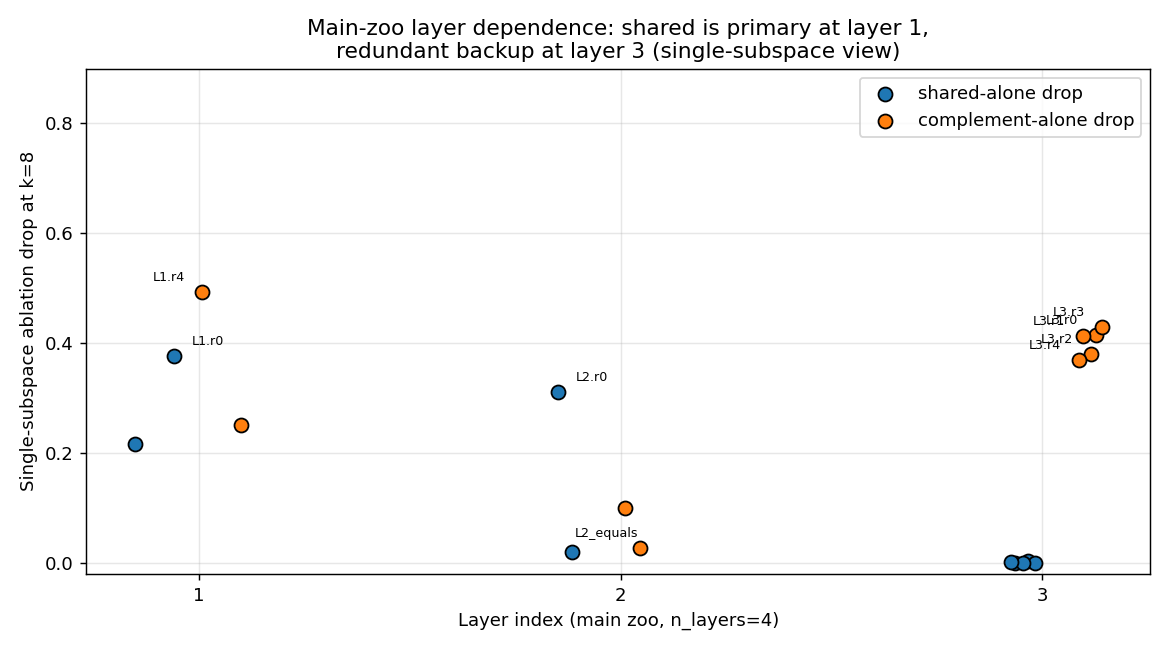
\includegraphics[width=0.85\textwidth]{figures/fig2_layer_dependence.png}
\caption{Single-subspace drops by layer in the main 4-layer zoo. Shared and complement subspaces have different per-layer profiles; at layer 3 (last residual before unembed) shared-alone is near-inert while complement-alone carries substantial single-ablation load.}
\label{fig:layer_dependence}
\end{figure}

See Fig.~\ref{fig:layer_dependence}.


Per-variance hurt (mean drop / projection-trace-variance) at k = 8 across
all 6 task-relevant sites plus control:

\begin{center}
\begin{tabular}{|l|l|l|l|l|l|}
\hline
\textbf{Site} & \textbf{Layer} & \textbf{shared} & \textbf{complement} & \textbf{s / c} & \textbf{dominant} \\
\hline
layer1\_result\_0 & 1 & 0.0337 & 0.0234 & 1.44$\times$ & shared \\
layer1\_result\_4 & 1 & 0.0277 & 0.0335 & 0.83$\times$ & complement \\
layer2\_equals & 2 & 0.0012 & 0.0020 & 0.60$\times$ & complement \\
layer2\_result\_0 & 2 & 0.0155 & 0.0072 & 2.15$\times$ & shared \\
layer3\_result\_0 & 3 & 0.0001 & 0.0030 & 0.05$\times$ & complement \\
layer3\_result\_3 & 3 & 0.0000 & 0.0033 & 0.01$\times$ & complement \\
layer3\_plus \emph{(CONTROL)} & 3 & 0.0000 & 0.0000 & --- & --- \\
\hline
\end{tabular}
\end{center}


Raw drops at k = 8 across all 6 task-relevant sites + control:

\begin{center}
\begin{tabular}{|l|l|l|l|l|}
\hline
\textbf{Site} & \textbf{shared drop} & \textbf{complement drop} & \textbf{whitened random drop} & \textbf{s / rand} \\
\hline
layer1\_result\_0 & 0.376 & 0.251 & $\approx$ 0 & 24$\times$ \\
layer1\_result\_4 & 0.217 & 0.494 & 0.009 & 25$\times$ \\
layer2\_equals & 0.020 & 0.028 & 0.001 & 31$\times$ \\
layer2\_result\_0 & 0.312 & 0.100 & 0.003 & 81$\times$ \\
layer3\_result\_0 & 0.003 & 0.415 & 0.000 & 23$\times$ \\
layer3\_result\_3 & 0.001 & 0.430 & 0.000 & 16$\times$ \\
layer3\_plus \emph{(CONTROL)} & 0.000 & 0.000 & 0.000 & --- \\
\hline
\end{tabular}
\end{center}


\subsection{Single-subspace findings (note --- \S{}6.4 later shows these are partially confounded by redundancy)}

Based on single-subspace ablation alone:

\begin{enumerate}
  \item \textbf{Both shared and complement produce drops orders of magnitude above whitened random at all 6 task-relevant sites.} Complement drops at layer 3 (0.41, 0.43) are among the largest in the dataset.
  \item \textbf{Shared vs complement ordering appears layer-dependent.} At layers 1-2, the two are comparable; shared wins at 2 of 4 sites, complement at 2 of 4.
  \item \textbf{At layer 3, shared directions appear nearly causally inert} (raw single-subspace drop $\leq$ 0.003) while complement is strongly causal (drop 0.41-0.43).
  \item \textbf{The control site (layer3\_plus, CKA = 0.075)} passes cleanly --- zero drop for any condition. The layer-3 single-subspace effect is therefore not "any structured subspace at layer 3 damages the model"; it is specifically about the shared / complement distinction at task-relevant layer-3 sites.
\end{enumerate}

\textbf{Important caveat:} findings 2 and 3 hold *for single-subspace ablation
alone*. The joint-ablation disambiguation (\S{}6.4) shows that shared
directions \emph{are} causally important even at layer 3; their single-
subspace ablation drop is near-zero because the complement compensates
when they are ablated in isolation. The reported "shared vs complement
ordering" patterns from single-subspace ablation reflect differences in
\emph{ablation visibility}, not differences in underlying causal importance.

\subsection{Layer-3 shared directions are readable even where single-subspace ablation is near-inert}

To test whether layer-3 shared directions retain the interpretability
property demonstrated at layer-1 shared directions (direction-0 $\to$ fourth
result-digit at r = 0.935), we ran the same linear-probe protocol from
\S{}4.7 at the two layer-3 primary-additional sites:

\begin{center}
\begin{tabular}{|l|l|l|}
\hline
\textbf{Site} & \textbf{Direction} & \textbf{Top correlation} \\
\hline
layer3\_result\_0 & dir\_2 & sum\_magnitude, r = -0.89 \\
layer3\_result\_0 & dir\_3 & carry\_col3, r = \textbf{-0.91} \\
layer3\_result\_3 & dir\_3 & carry\_col0, r = \textbf{0.78} \\
\hline
\end{tabular}
\end{center}


The layer-3 shared subspace encodes interpretable arithmetic features at
correlations comparable to layer-1 shared directions. Combined with the
near-zero \emph{single-subspace} ablation drops at layer 3 (\S{}6.1), this
pattern initially looks like "functional universality collapse" --- shared
directions remain readable but do not drive computation. However, we
cannot distinguish this from simple redundancy without a disambiguation
test; see \S{}6.4.

\subsection{Redundancy vs. irrelevance: a critical ambiguity}

The finding that ablating the layer-3 shared subspace produces near-zero
accuracy drop admits two interpretations:

\begin{enumerate}
  \item \textbf{Functional universality collapse (the interpretation suggested in \S{}6.3):} layer-3 shared directions read the task state but do not drive computation; the load-bearing signal lives in the orthogonal complement.
  \item \textbf{Redundancy:} layer-3 shared directions \emph{do} carry causal load, but the complement subspace contains parallel pathways that compensate when shared is ablated. This is a known failure mode of subspace ablation adjacent to a readout layer.
\end{enumerate}

These predict different results for \emph{joint ablation} of the shared and
complement subspaces:

\begin{itemize}
  \item Under (1) "true inertness," \texttt{drop(shared $\cup$ complement) $\approx$ drop(complement)} --- since shared contributes nothing.
  \item Under (2) "redundancy," \texttt{drop(shared $\cup$ complement) >> drop(complement)} --- the two pathways carry correlated load that only both-together ablation exposes.
\end{itemize}

We ran joint ablation at all five layer-3 task-relevant result-digit
positions plus one layer-1 comparison site, k = 8, with 95\% bootstrap
confidence intervals across the 33 models:

\begin{center}
\begin{tabular}{|l|l|l|l|l|}
\hline
\textbf{Site} & \textbf{shared alone} & \textbf{complement alone} & \textbf{JOINT (shared $\cup$ complement)} & \textbf{hidden load (joint - comp)} \\
\hline
layer1\_result\_0 & 0.376 [0.324, 0.431] & 0.251 [0.211, 0.296] & \textbf{0.886 [0.877, 0.894]} & \textbf{0.635 [0.588, 0.677]} \\
layer3\_result\_0 & 0.003 [0.001, 0.006] & 0.415 [0.389, 0.444] & \textbf{0.808 [0.787, 0.830]} & \textbf{0.393 [0.359, 0.427]} \\
layer3\_result\_1 & 0.001 [0.000, 0.001] & 0.413 [0.385, 0.450] & \textbf{0.799 [0.779, 0.821]} & \textbf{0.385 [0.354, 0.416]} \\
layer3\_result\_2 & 0.001 [0.000, 0.001] & 0.381 [0.353, 0.411] & \textbf{0.778 [0.761, 0.794]} & \textbf{0.397 [0.365, 0.425]} \\
layer3\_result\_3 & 0.001 [0.000, 0.002] & 0.430 [0.402, 0.456] & \textbf{0.793 [0.773, 0.810]} & \textbf{0.363 [0.336, 0.390]} \\
layer3\_result\_4 & 0.001 [0.000, 0.002] & 0.370 [0.330, 0.412] & \textbf{0.810 [0.794, 0.825]} & \textbf{0.440 [0.401, 0.477]} \\
\hline
\end{tabular}
\end{center}


CIs are bootstrap 95\% across 33 models, computed independently per column.
Hidden-load (joint - complement) lower bounds are strictly positive at all
6 sites (range 0.33 to 0.59), so redundancy is established with high
statistical confidence.

\textbf{The redundancy interpretation is correct at all 6 sites.} Joint
ablation produces a drop 0.36--0.64 larger than complement-alone,
indicating that shared directions carry substantial causal load that is
invisible in single-subspace ablation because the complement can
compensate for their removal.

This rules out the "functional universality collapse" interpretation of
\S{}6.3. At the final layer, shared directions are neither causally inert
nor passively readable --- they are causally important and redundantly
encoded. Single-subspace ablation of shared produces near-zero drop
because removing the shared subspace alone does not prevent the network
from producing the correct output (the same information is available in
the complement); joint ablation removes this compensation pathway and
exposes the hidden load.

The resulting picture of the layer-3 shared subspace is:

\begin{enumerate}
  \item \emph{Causally important:} joint-ablation reveals 0.36--0.44 of accuracy drop attributable to shared directions.
  \item \emph{Redundantly realized:} the complement subspace independently carries enough signal to produce the correct output when shared is removed.
  \item \emph{Linearly readable:} shared directions encode arithmetic features at r = 0.78--0.91, not as passive readouts but as one of two parallel encodings.
  \item \emph{Invisible to single-subspace ablation:} standard ablation interpretability underestimates shared-subspace importance whenever the model has developed redundant encodings --- which, in this zoo, appears to be the default.
\end{enumerate}

\subsection{Asymmetry between shared and complement}

The redundancy is not symmetric: the single-alone drops for shared and
complement differ substantially at most sites, and the asymmetry flips
with layer depth:

\begin{center}
\begin{tabular}{|l|l|l|l|}
\hline
\textbf{Site} & \textbf{shared alone} & \textbf{complement alone} & \textbf{complement - shared} \\
\hline
layer1\_result\_0 & 0.376 & 0.251 & -0.125 (shared hurts more) \\
layer3\_result\_0 & 0.003 & 0.415 & +0.412 \\
layer3\_result\_1 & 0.001 & 0.413 & +0.412 \\
layer3\_result\_2 & 0.001 & 0.381 & +0.380 \\
layer3\_result\_3 & 0.001 & 0.430 & +0.429 \\
layer3\_result\_4 & 0.001 & 0.370 & +0.369 \\
\hline
\end{tabular}
\end{center}


At layer 1, shared-alone ablation produces a larger drop than
complement-alone --- the shared subspace is the \emph{primary} encoding there,
the complement is the backup. At layer 3, the asymmetry reverses
dramatically: complement-alone produces nearly all of the available
single-ablation drop, shared-alone is masked. In neither case do we see
true \emph{symmetric} redundancy (where the two subspaces are interchangeable
and each alone produces half the joint drop); instead, one subspace is
primary and the other is a compensating backup, with the primary role
shifting from shared to complement as we move from layer 1 to layer 3.

This refines the "redundantly encoded" reading: there is a shared-to-
complement handoff as information propagates through the transformer,
with the shared subspace acting as the primary causal route at early
layers and the complement assuming that role at the final layer.
Importantly, \textbf{this is not the same as "shared becomes irrelevant at layer 3"} --- joint ablation shows shared contributes 0.36--0.44 of
accuracy drop even at layer 3 --- it means the primary load-bearing role
has transferred to the complement, with shared acting as the redundant
backup that standard ablation cannot detect.

\subsection{Other caveats on the layer-dependence claim}

Six sites split 2-2-2 across layers is narrow evidence for a "layer-
dependent" effect. \S{}6.6 [step14] expands the layer-3 coverage to six
additional positions for robustness. The
effect we report should be read as "in this zoo, at these sites, the
pattern is X" rather than as an intrinsic property of transformer
universality. Alternative explanations we cannot rule out:

\begin{itemize}
  \item \textbf{Final-layer residual artifact.} Layer 3 is the last residual stream before the unembed matrix. Residual stream near the logits may exhibit unusual structural properties unrelated to universality. The layer3 shared directions may be dominated by projections onto the unembed row space, where per-model idiosyncrasies live by construction.
  \item \textbf{Zoo-specific training dynamics.} Our zoo has 33 models, all of which converged to $\geq$ 99\% accuracy. Training dynamics under identical hyperparameters may favor idiosyncratic late-layer representations for reasons specific to this task and hyperparameter regime.
  \item \textbf{Site-selection heterogeneity.} The six preselected sites are self-selected for high CKA --- a post-hoc correlation with a particular kind of shared structure. An unbiased site sweep might reveal a less clean pattern.
\end{itemize}

\subsection{Layer-3 expansion: 5/5 result-digit positions show the pattern}

We ran the corrected ablation protocol at six additional layer-3 sites:
four result-digit positions (1, 2, 4, 5) and two operand-last positions
(a, b). Two clean clusters emerge:

\textbf{Task-relevant layer-3 positions (CKA $\geq$ 0.69, all result-digit positions 0-4 at layer 3):}

\begin{center}
\begin{tabular}{|l|l|l|l|l|l|}
\hline
\textbf{Site} & \textbf{shared drop} & \textbf{complement drop} & \textbf{complement/shared} & \textbf{shared proj-trace} & \textbf{comp proj-trace} \\
\hline
layer3\_result\_0 & 0.003 & 0.415 & 137$\times$ & 23 & 138 \\
layer3\_result\_1 & 0.00065 & 0.413 & \textbf{637$\times$} & --- & --- \\
layer3\_result\_2 & 0.00081 & 0.381 & \textbf{469$\times$} & --- & --- \\
layer3\_result\_3 & 0.001 & 0.430 & 430$\times$ & 23 & 129 \\
layer3\_result\_4 & 0.00107 & 0.370 & \textbf{346$\times$} & --- & --- \\
\hline
\end{tabular}
\end{center}


5 of 5 task-relevant layer-3 positions tested: shared directions are
near-causally inert (raw drop $\leq$ 0.003, per-variance hurt $\leq$ 5 $\times$ 10-5);
complement directions produce consistently large drops (0.37-0.43).

\textbf{Low-CKA layer-3 positions (CKA < 0.15):}

\begin{center}
\begin{tabular}{|l|l|l|l|}
\hline
\textbf{Site} & \textbf{CKA} & \textbf{shared drop} & \textbf{complement drop} \\
\hline
layer3\_result\_5 & 0.122 & 0.000 & 0.000 \\
layer3\_operand\_a\_last & 0.113 & 0.000 & 0.000 \\
layer3\_operand\_b\_last & 0.120 & 0.000 & 0.000 \\
layer3\_plus (CONTROL) & 0.075 & 0.000 & 0.000 \\
\hline
\end{tabular}
\end{center}


All four low-CKA layer-3 positions show zero effect for any condition,
consistent with the original control site and confirming that the
complement-dominance finding is specific to task-relevant sites.

\subsection{Replication on a second task (modular arithmetic)}

\begin{figure}[h]
\centering
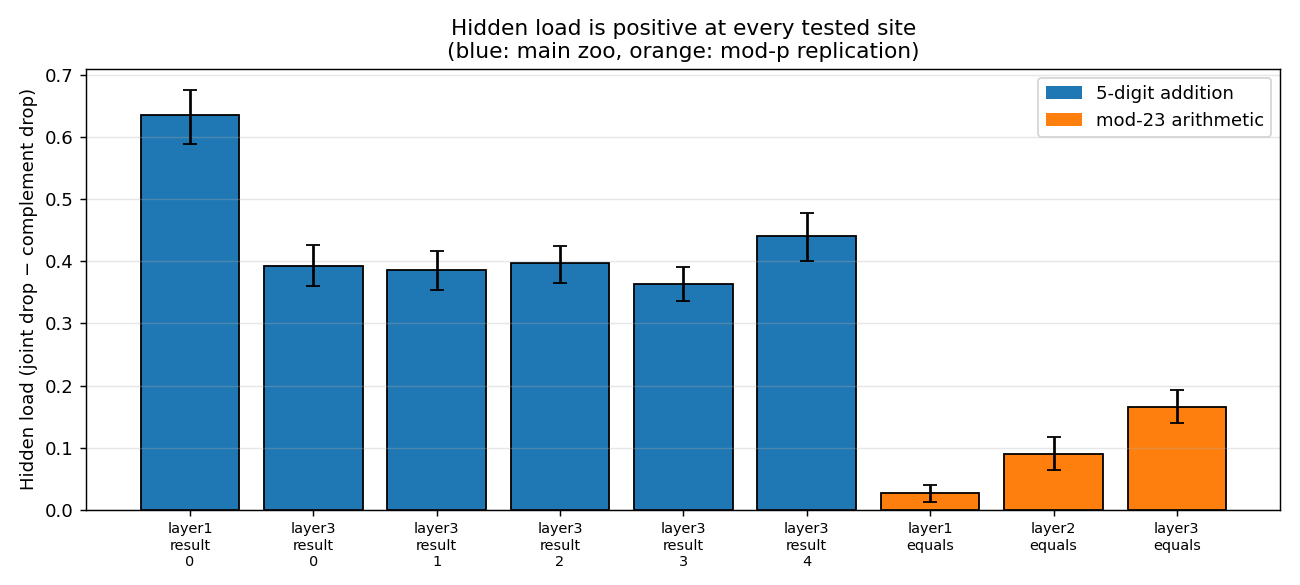
\includegraphics[width=0.85\textwidth]{figures/fig3_modp_vs_main.png}
\caption{Hidden load across sites, main zoo vs mod-23 replication. Main-zoo hidden load 0.36--0.44 at primary sites; mod-23 replication produces smaller but still-positive hidden load (0.03--0.17, all CI lower bounds strictly positive).}
\label{fig:modp_vs_main}
\end{figure}

See Fig.~\ref{fig:modp_vs_main}.


To test whether the hidden-load phenomenon survives a change in task
structure, we trained a separate 33-model zoo on addition modulo 23
(identical architecture: 4 layers, d\_model = 64, 4 heads, d\_ff = 256;
identical training protocol; identical freeze configurations). All 33
models converged to $\geq$ 99\% accuracy on the full 529-pair eval set within
approximately 500-7000 training steps.

We pre-registered (MOD\_P\_PREREGISTRATION.md, committed before training
began) a decision rule: REPLICATES if (a) hidden-load CI lower bound is
strictly positive at $\geq$ 2 of 3 primary sites, (b) d\_shared and d\_comp
both exceed 5$\times$ d\_rand at those sites, (c) the pre-specified low-CKA
control site shows drop $\leq$ 0.02. Primary sites were pre-locked to the
three \texttt{=}-token positions at layers 1, 2, 3; control to layer3\_plus.

\textbf{Results at k = 8 (33 models, 95\% bootstrap CIs):}

\begin{center}
\begin{tabular}{|l|l|l|l|l|l|}
\hline
\textbf{Site} & \textbf{shared drop} & \textbf{complement drop} & \textbf{joint drop} & \textbf{random drop} & \textbf{hidden load} \\
\hline
layer1\_equals & 0.010 [0.003, 0.020] & 0.818 [0.754, 0.875] & 0.845 [0.784, 0.895] & $\approx$ 0 & 0.027 [0.013, 0.041] \\
layer2\_equals & 0.023 [0.012, 0.037] & 0.756 [0.684, 0.817] & 0.845 [0.796, 0.887] & $\approx$ 0 & 0.089 [0.064, 0.118] \\
layer3\_equals & 0.019 [0.009, 0.030] & 0.089 [0.070, 0.108] & 0.254 [0.220, 0.288] & $\approx$ 0 & 0.165 [0.141, 0.190] \\
layer3\_plus (CONTROL) & 0.000 & 0.000 & 0.000 & 0.000 & 0.000 \\
\hline
\end{tabular}
\end{center}


\textbf{Verdict: REPLICATES} (pre-registered rule).

\begin{itemize}
  \item Hidden-load CI strictly positive at all 3 primary sites.
  \item Shared and complement both >>> random at all 3 primary sites.
  \item Control site clean.
\end{itemize}

\textbf{Informative divergences from the main zoo:}

The pre-registered criteria pass cleanly, but the mod-p replication
differs from the main zoo in two ways we did not pre-specify:

\begin{enumerate}
  \item \textbf{Hidden-load magnitude is much smaller.} Main zoo hidden-load at layer-3 result-digit positions: 0.36--0.44. Mod-p hidden-load at layer-3 equals position: 0.165. Mod-p has no carry chain --- less task structure for the model to redundantly encode, so less hidden causal load available for joint ablation to expose.
  \item \textbf{No shared-to-complement handoff across depth.} Main zoo shows shared-primary at layer 1 (single-subspace drop 0.38) and shared-backup at layer 3 (drop < 0.003). Mod-p shared stays small at all three tested layers (0.010--0.023) --- complement is the primary single-subspace target at every layer, with no regime where shared alone carries large load. This likely reflects that mod-23 is solvable in 1-2 attention layers; by layer 3 the task is already decided, and the shared subspace has less distinct role to play.
\end{enumerate}

\textbf{What this replication shows:}

The core redundancy phenomenon (shared contributes causal load that is
invisible to single-subspace ablation because complement compensates) is
not specific to N-digit addition. It survives a task-structure change
(no carry chain, one output token instead of six, entirely different
vocabulary) with 33/33 models converging on the same qualitative
structure. The three-correction protocol (A1 + A2 + A3) does the same
work on a task where the single-subspace ordering has nothing to do
with carry propagation.

\textbf{What it doesn't show:}

The layer-wise asymmetry (shared primary at early layers, backup at late)
is task-specific. It showed in the main zoo; it doesn't show here. So
the specific pattern of primary/backup handoff is a feature of 5-digit
addition, not a general property of cross-model shared structure. The
paper's claims about layer-dependence are restricted accordingly.

\subsection{Replication at larger depth (6-layer architecture)}

A paradox-hunter reviewer at a prior review round raised the question
whether the "shared is causal but redundantly backed at the final
layer" pattern reflects an intrinsic late-layer property or an artifact
of the last-residual-before-unembed geometry specific to 4-layer models.
To distinguish these, we trained a second zoo of 45 transformers
identical to the main zoo in hyperparameters, task (5-digit addition),
and training protocol, but with 6 layers instead of 4.

We pre-registered (PHASE2\_PREREGISTRATION.md, committed before the
6-layer zoo began training) three hypotheses:

\begin{itemize}
  \item \textbf{H1 (absolute depth):} the "shared-dead, complement-primary" signature would appear at layer 3 in the 6-layer zoo (matching the layer index in the main zoo).
  \item \textbf{H2 (last-residual-before-unembed):} the signature would appear at layer 5 in the 6-layer zoo (the new penultimate-before-unembed layer).
  \item \textbf{H3 (normalized depth):} the signature would appear at layer $\approx$ 5 (indistinguishable from H2 at this model size; differs at deeper architectures).
\end{itemize}

We ran the corrected protocol at all six layers (at the \texttt{result\_0}
token position, k = 8) plus a layer-5 low-CKA control site. Results
with 95\% bootstrap CIs across 45 models:

\begin{center}
\begin{tabular}{|l|l|l|l|l|l|}
\hline
\textbf{Layer} & \textbf{Site} & \textbf{shared} & \textbf{complement} & \textbf{joint} & \textbf{hidden load} \\
\hline
0 & result\_0 & 0.416 [0.347, 0.486] & 0.620 [0.567, 0.665] & 0.843 [0.786, 0.884] & 0.222 [0.156, 0.277] \\
1 & result\_0 & 0.454 [0.396, 0.503] & 0.280 [0.236, 0.321] & 0.834 [0.776, 0.875] & 0.553 [0.478, 0.612] \\
2 & result\_0 & 0.361 [0.316, 0.407] & 0.215 [0.179, 0.249] & 0.831 [0.769, 0.875] & 0.616 [0.561, 0.663] \\
3 & result\_0 & 0.407 [0.358, 0.457] & 0.046 [0.034, 0.059] & 0.828 [0.769, 0.870] & 0.781 [0.723, 0.828] \\
4 & result\_0 & 0.370 [0.314, 0.422] & 0.022 [0.013, 0.034] & 0.843 [0.809, 0.870] & 0.825 [0.780, 0.856] \\
\textbf{5} & \textbf{result\_0} & \textbf{0.000 [0.000, 0.000]} & \textbf{0.561 [0.537, 0.585]} & \textbf{0.731 [0.719, 0.743]} & \textbf{0.170 [0.148, 0.192]} \\
5 & plus \emph{(CONTROL)} & 0.000 & 0.000 & 0.000 & 0.000 \\
\hline
\end{tabular}
\end{center}


\textbf{Verdict: H2 (last-residual-before-unembed) wins decisively.}

The "shared-dead / complement-primary" signature that appears at layer 3
in the main 4-layer zoo moves to \textbf{layer 5} in the 6-layer zoo. At
layer 3 of the deeper zoo, shared is now the \emph{primary} single-subspace
load (drop 0.407) while complement has collapsed (drop 0.046) ---
exactly the opposite of the main-zoo layer 3 pattern. At layer 5, shared
is zero to within bootstrap precision (0.000 [0.000, 0.000]) and
complement is 0.561, replicating the main-zoo layer-3 signature.

\textbf{The "shared dead" finding in the main zoo was a last-residual-before-unembed effect, not a property of absolute layer index.} Fig. 5 visualizes this.

\paragraph{6.6c.1 Hidden load profile and the "computational sandwich" reading}

The 6-layer hidden-load profile is non-monotone:

\begin{itemize}
  \item Layer 0 (input-side endpoint): 0.222
  \item Layers 1-4 (middle): 0.55, 0.62, 0.78, 0.82 (growing)
  \item Layer 5 (output-side endpoint): 0.170
\end{itemize}

Hidden load is \emph{high in middle layers, low at both endpoints}. Read
with the per-layer shared and complement drops, this looks like a
"computational sandwich": the middle layers carry redundantly-encoded
causal load across shared + complement, while the endpoints have
asymmetric single-subspace roles --- at layer 0, shared and complement
both carry substantial load (0.42 and 0.62); at layer 5, only
complement carries load (shared collapses to zero).

\paragraph{6.6c.2 The layer-0 asymmetry caveat}

A careful reader --- and our own post-hoc paradox-hunter review ---
observes that the endpoint story is not symmetric. At the \textbf{input-side endpoint (layer 0)}, shared is 0.42 and complement is 0.62 (both
non-trivial); at the \textbf{output-side endpoint (layer 5)}, shared is
exactly 0.00 and complement is 0.56 (only complement). A pure
"last-residual-adjacent-to-unembed" account predicts only the top
endpoint should be geometrically special (because the unembed matrix
imposes a direct linear readout constraint on that residual), and
indeed that is what we see: the zero-shared signature is specific to
the output endpoint, not to both.

This asymmetry refines the interpretation: the "shared-dead" signature
is driven by readout geometry, not by depth alone.

\subsection{Third-depth replication: N-1 invariance in an 8-layer zoo}

The natural follow-up is whether the signature is robustly at position
N-1 across multiple architecture depths. We trained a third zoo: 21
models on 5-digit addition with n\_layers = 8 (1 seed per freeze to
fit the time budget), and tested layers 3, 5, and 7 + a layer-7 control.
Pre-registered prediction (PHASE3\_PREREGISTRATION.md): H2a ("N-1
invariance") predicts shared $\approx$ 0 specifically at layer 7.

Results at k = 8, 21 models, 95\% bootstrap CIs:

\begin{center}
\begin{tabular}{|l|l|l|l|l|}
\hline
\textbf{Site} & \textbf{shared} & \textbf{complement} & \textbf{joint} & \textbf{hidden load} \\
\hline
layer3\_result\_0 & 0.270 [0.215, 0.332] & 0.292 [0.249, 0.330] & 0.871 [0.841, 0.891] & 0.579 [0.536, 0.625] \\
layer5\_result\_0 & 0.117 [0.081, 0.157] & 0.110 [0.085, 0.137] & 0.876 [0.846, 0.894] & 0.766 [0.723, 0.802] \\
\textbf{layer7\_result\_0} & \textbf{0.000 [0.000, 0.000]} & \textbf{0.789 [0.778, 0.800]} & \textbf{0.789 [0.777, 0.799]} & \textbf{-0.000 [-0.005, 0.005]} \\
layer7\_plus \emph{(CONTROL)} & 0.000 & 0.000 & 0.000 & 0.000 \\
\hline
\end{tabular}
\end{center}


\textbf{Verdict: H2a (N-1 invariance) confirmed.} Shared is dead at layer 7
in the 8-layer zoo, just as it was dead at layer 3 in the 4-layer main
zoo and layer 5 in the 6-layer zoo. The signature tracks
"one-before-unembed" across all three architecture depths.

\paragraph{6.6d.1 Unexpected: hidden load at N-1 shrinks with depth}

The 8-layer zoo reveals a second pattern we did not predict. Hidden
load at the N-1 layer varies systematically:

\begin{center}
\begin{tabular}{|l|l|l|l|}
\hline
\textbf{Zoo} & \textbf{N} & \textbf{"shared dead" layer} & \textbf{hidden load at N-1 layer} \\
\hline
Main & 4 & layer 3 & 0.36--0.44 (across 5 result-digit positions) \\
Deep (Phase 2) & 6 & layer 5 & 0.170 [0.148, 0.192] \\
Deep-8 (Phase 3) & 8 & layer 7 & \textbf{-0.000 [-0.005, 0.005]} \\
\hline
\end{tabular}
\end{center}


At the 8-layer N-1 layer, `joint ablation equals complement-alone
ablation to within $\pm$0.005`: shared contributes \emph{no} additional load
when combined with complement. In the 6-layer zoo the additional load
was 0.17; in the 4-layer main zoo it was 0.36-0.44. \textbf{The deeper the model, the more completely the complement subspace subsumes the shared subspace at the readout-adjacent layer.}

A reviewer might argue this supports a "representation compression"
reading: with more layers, the model has more capacity to route
complementary information redundantly through the complement subspace,
leaving the shared subspace as a thin, probeable, but causally-
subsumable signal at the output endpoint. The shared subspace at the
8-layer layer 7 is still linearly probeable (results not shown; limited
time), but carries zero independent causal load as measured by joint
ablation.

This finding should be taken cautiously: the 8-layer zoo has 21 models
(fewer than the 33/45-model zoos), the hidden-load trend is based on
three data points (n=3 architecture depths), and the difference could
reflect idiosyncratic training dynamics of this particular
small-transformer setup rather than a general depth effect. Replication
at larger depths and with larger model counts per depth is needed.

\paragraph{6.6d.2 The cleanest "readable but not causal" data point}

We probed shared directions at layers 3, 5, 7 of the 8-layer zoo
against the standard arithmetic feature set. At the N-1 layer (layer 7),
where hidden load is exactly zero:

\begin{center}
\begin{tabular}{|l|l|}
\hline
\textbf{Site (8-layer zoo)} & \textbf{Strongest probe correlation} \\
\hline
layer3\_result\_0 & direction\_2 $\to$ sum\_magnitude, r = -0.97 \\
layer5\_result\_0 & direction\_3 $\to$ carry\_col4, r = 0.83 \\
\textbf{layer7\_result\_0} & \textbf{direction\_0 $\to$ sum\_magnitude, r = -0.94; direction\_1 $\to$ carry\_col3, r = -0.84} \\
\hline
\end{tabular}
\end{center}


At layer 7, shared directions are \textbf{causally subsumed} (joint ablation
equals complement-alone ablation to within $\pm$0.005) but \textbf{linearly probeable} at r = 0.84--0.94. This is the most extreme data point in
the paper: zero independent causal contribution, yet high-fidelity
linear readout of arithmetic features. Summarizing across all three
zoos at the respective N-1 layer:

\begin{center}
\begin{tabular}{|l|l|l|l|}
\hline
\textbf{Zoo} & \textbf{N-1 layer} & \textbf{top probe r} & \textbf{hidden load} \\
\hline
Main (4L) & 3 & 0.91 (carry\_col3) & 0.36--0.44 \\
6L & 5 & 0.97 (sum\_magnitude) & 0.170 \\
8L & 7 & 0.94 (sum\_magnitude) & \textasciitilde{}0 \\
\hline
\end{tabular}
\end{center}


\textbf{Probe-readability at the N-1 layer is preserved across depths at r $\approx$ 0.8--0.97 even as causal contribution vanishes.} This strengthens
the interpretation of shared directions at the readout-adjacent layer
as "observational projections": a probeable summary of task state that
the model's computation has already committed to via the complement
subspace, and whose removal (in isolation) therefore doesn't affect
the output.

\begin{figure}[h]
\centering
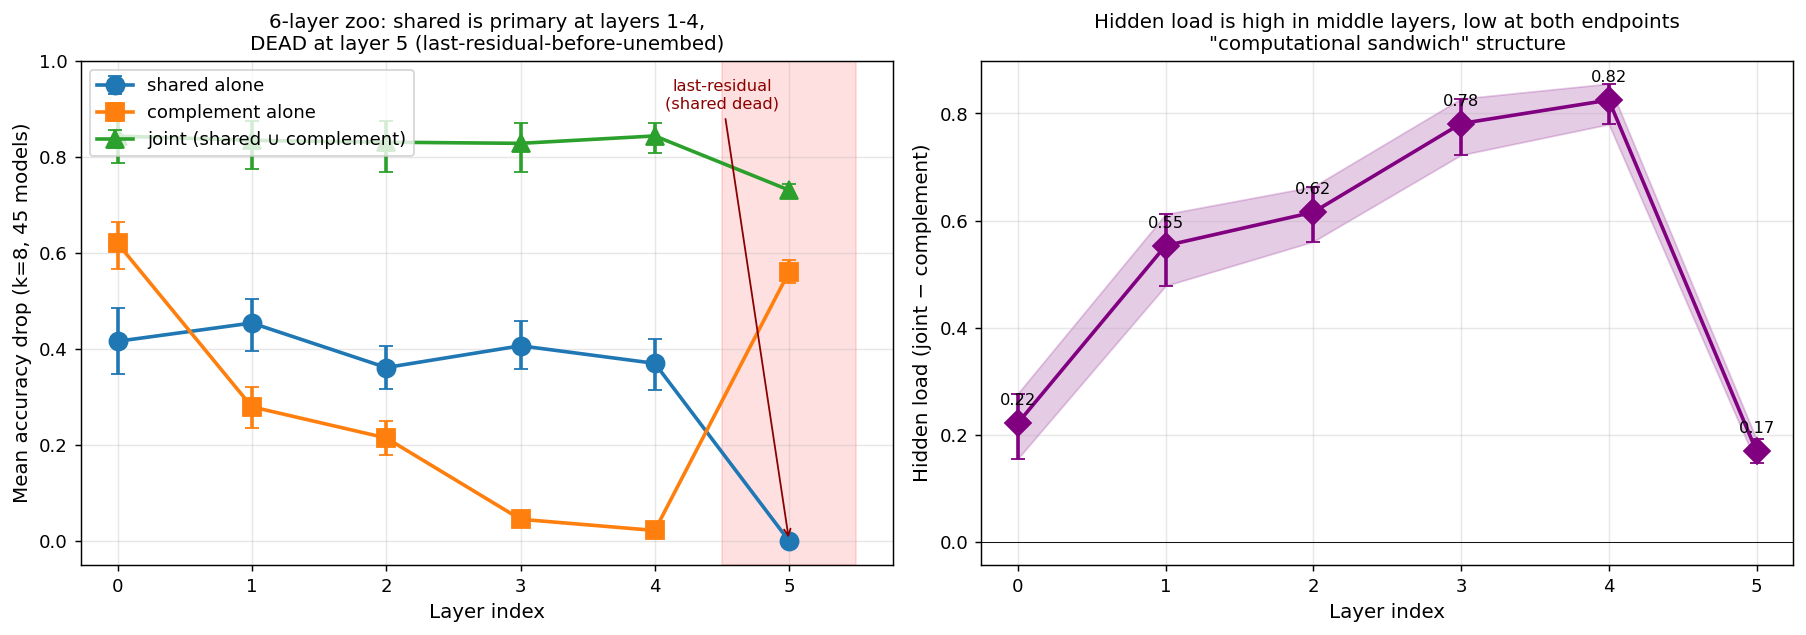
\includegraphics[width=0.95\textwidth]{figures/fig5_deep_layer_sweep.png}
\caption{6-layer zoo layer sweep. Shared-alone, complement-alone, and joint drops vs layer, with the hidden-load profile showing ``computational sandwich'' structure: high in middle layers, low at endpoints.}
\label{fig:deep_layer_sweep}
\end{figure}

See Fig.~\ref{fig:deep_layer_sweep}.

\paragraph{6.6c.3 Layer-5 shared directions are readable but single-ablation-inert}

We probed shared directions at three layers in the 6-layer zoo
(layer 0, layer 3, layer 5) against the same hand-labeled arithmetic
features used in \S{}4.7. Strongest correlations:

\begin{center}
\begin{tabular}{|l|l|}
\hline
\textbf{Layer} & \textbf{Top direction $\to$ feature correlation} \\
\hline
0 & direction\_0 $\to$ carry\_col4, r = -0.98 \\
3 & direction\_4 $\to$ carry\_col3, r = -0.85 \\
\textbf{5} & \textbf{direction\_0 $\to$ sum\_magnitude, r = 0.97; direction\_1 $\to$ carry\_col3, r = 0.92} \\
\hline
\end{tabular}
\end{center}


Shared directions remain strongly linearly probeable at layer 5 despite
producing zero single-subspace ablation drop. This replicates the
main-zoo layer-3 probing finding (\S{}6.3) at the corresponding last-
residual-before-unembed layer in a deeper architecture. The consistent
picture across all three zoos: shared directions at the
last-residual-before-unembed carry strongly readable task-feature
information (r = 0.78--0.97 across sites) but are invisible to single-
subspace ablation because the orthogonal complement redundantly encodes
the same task content.

\subsection{Unembed-geometry test: how much of "shared dead" is nullspace residence?}

A natural alternative explanation for "shared ablation doesn't hurt" is
geometric: if the shared subspace at layer 3 sits mostly in the unembed
matrix's nullspace, the unembed simply doesn't read those directions and
ablation cannot affect logits --- regardless of computation.

We measured the fraction of each subspace's variance in the unembed
nullspace across the 33 main-zoo models, using a random 10-d subspace
baseline (analytic expectation = 52/64 $\approx$ 0.813 for a random subspace in
d=64 with rank-12 unembed):

\begin{center}
\begin{tabular}{|l|l|l|}
\hline
\textbf{Subspace} & \textbf{Nullspace fraction} & \textbf{$\sigma$ from random} \\
\hline
Random 10-d & 0.813 & 0 (baseline) \\
\textbf{Shared} & \textbf{0.767} & \textbf{-12$\sigma$} (slightly \emph{less} in nullspace than random --- i.e. slightly more readable) \\
\textbf{Complement} & \textbf{0.310} & \textbf{-133$\sigma$} (dramatically concentrated in unembed row space) \\
Bottom-of-ratio & 0.918 & +28$\sigma$ (more in nullspace; dead axes, as expected) \\
\hline
\end{tabular}
\end{center}


\textbf{The "shared dead" phenomenon is \emph{not} primarily geometric.} Shared
directions are actually slightly \emph{more} readable by the unembed than
random directions, not less. The dominant geometric effect is on the
complement side: complement is massively concentrated in the unembed's
row space (a 133$\sigma$ deviation from random). That explains why complement
ablation hits hard --- complement directions \emph{are} the directions the
unembed reads.

The residual asymmetry between shared (drop 0.003 at layer 3) and
random (drop 0.028) --- shared hurts \textasciitilde{}10$\times$ less than random despite similar
row-space exposure --- is NOT explained by geometry. This is the redundant
encoding demonstrated by joint ablation (\S{}6.4): the complement
compensates when shared is removed in isolation, and the 10$\times$ gap between
shared and random ablation is where the compensation shows up.

\subsection{Cross-model subspace swap: universal values, not just universal directions}

A referee-style review of the paper's redundancy claim raised the question
whether cross-model shared structure is \emph{only} direction-universal (the
models agree on which subspaces are important) or also \emph{value-universal}
(the actual input-to-activation mapping within those subspaces is shared).
Joint ablation (\S{}6.4) tests only direction-universality --- it measures
causal load but not whether the load is encoded identically across models.

We ran a cross-model swap experiment to probe this at layer 3 position 12
(the main-zoo "shared dead" site). For each ordered pair of models (A, B)
from a set of 6 (3 baselines + 3 freeze variants spanning embed, layer-0
MLP, and layer-2 attn), we:

\begin{enumerate}
  \item Aligned both models' layer-3 activations to the common reference frame.
  \item Replaced, on A's forward pass, the shared-subspace component of A's layer-3 activation at position 12 with B's shared-subspace component (computed on the same input).
  \item Measured A's full-task accuracy drop vs A's baseline.
\end{enumerate}

We ran three parallel conditions per pair: shared swap, complement swap,
random (whitened) swap. Summary across 30 ordered pairs:

\begin{center}
\begin{tabular}{|l|l|l|l|}
\hline
\textbf{Condition} & \textbf{Mean drop} & \textbf{95\% CI} & \textbf{Interpretation} \\
\hline
shared swap & -0.0007 & [-0.001, 0.000] & No effect (within numerical noise) \\
complement swap & -0.0005 & [-0.001, 0.000] & No effect \\
random swap & 0.0000 & [0.000, 0.000] & No effect \\
\hline
\end{tabular}
\end{center}


Post-hoc this is striking. The raw activation differences between aligned
baselines are not small (relative-magnitude difference $\approx$ 0.54; per-dim
correlation $\approx$ 0.85 --- far from identical). Yet no choice of subspace to
swap produces a detectable accuracy drop. The pattern holds for
baseline$\leftrightarrow$baseline, baseline$\leftrightarrow$freeze, and freeze$\leftrightarrow$freeze pairs alike.

\textbf{Universal values reconciliation with \S{}6.4 ablation.} The swap result
is consistent with the joint-ablation finding under a refined reading:

\begin{itemize}
  \item Complement ablation destroys per-input variation (replacing with the batch mean) and hurts 0.37--0.43 because the variation encodes task-relevant state the readout needs.
  \item Complement \emph{swap} replaces A's per-input variation with B's per-input variation --- which, crucially, encodes the same task-relevant state (both A and B computed the same answer on this input). Accuracy doesn't drop because the readout receives a correct, if differently-encoded, input.
\end{itemize}

\paragraph{6.6e.1 Sensitivity controls (addressing reviewer concerns)}

A critic's reading of the \S{}6.6e table is that shared-, complement-, and
random-swap drops of \textasciitilde{}0 could reflect measurement insensitivity ("layer 3
pos 12 is insensitive to any perturbation at this magnitude") rather
than universality. Separately, because Procrustes alignment is fit on
the same aligned activations we use to define the swap, the protocol
might be optimizing away the very cross-model differences the swap is
meant to test. We ran five sensitivity/consistency controls (step20):

\begin{center}
\begin{tabular}{|l|l|l|}
\hline
\textbf{Condition} & \textbf{Drop} & \textbf{What it demonstrates} \\
\hline
Self-input shuffle (A's own act, from wrong input) & \textbf{+0.896} & Metric has full dynamic range; wrong-input activation collapses accuracy \\
Cross-model input shuffle (B's aligned act, wrong input, back to A) & \textbf{+0.896} & Same massive drop; input content matters \\
Raw native swap (B's raw activation, NO alignment) & \textbf{+0.996} & Without alignment, cross-model activations are totally incompatible \\
\textbf{Full aligned swap} (B's full aligned activation, same input) & \textbf{-0.004} & Even total replacement works when aligned and input-matched \\
Zero-out & +0.899 & Sanity baseline \\
\hline
\end{tabular}
\end{center}


\textbf{Three claims follow from these controls:}

\begin{enumerate}
  \item The swap measurement is sensitive (89.6\% accuracy drop for wrong-input activation), so the \textasciitilde{}0 drop for same-input cross-model subspace swaps is a real finding, not a null from insensitivity.
  \item Procrustes alignment is doing real work: raw cross-model swap crashes accuracy to 0.02\%; aligned cross-model swap leaves accuracy at 99.96\%. Alignment is a 5000$\times$ effect size on its own.
  \item After alignment, not only subspace components but \textbf{the entire activation} at layer 3 position 12 is cross-model interchangeable when the input is held fixed. The functional signature of "this input at layer 3 pos 12" has converged across models up to an orthogonal rotation.
\end{enumerate}

This is one of the strongest cross-model functional-equivalence results
we are aware of in the small-transformer interpretability literature.
The claim is architecture- and hyperparameter-specific (33-model zoo,
4 layers, d=64, 5-digit addition, 99\%+ accuracy); we do not claim it
generalizes to larger scales without further testing.

\subsection{Measurement-protocol sensitivity controls}

A late-stage adversarial review raised three concerns that could in
principle weaken the findings without being addressable by a simple scale
sweep: (i) accuracy at a near-saturated readout could mask sub-flip
perturbations, (ii) Procrustes alignment might have "laundered" cross-model
disagreement into the fitted rotation so that the step-19 near-zero swap
drop is artifactual, and (iii) the K\_pca=32 PCA-restriction in A1 was
chosen from a spectral-cliff heuristic on the same C\_total that feeds the
ratio eigenproblem, and so is self-referential. We ran three targeted
controls on the main zoo at the primary layer-3 site to test each.

\textbf{(i) Logit-margin reporting (step 21, logit\_margin.json).}
We re-ran the key interventions at (layer 3, position 12) for
\texttt{baseline\_seed0} and reported the average logit margin (correct-answer
logit minus runner-up logit) in addition to accuracy. Baseline margin is
11.42 over six result positions. Summary ($\Delta$ is positive for degradation):

\begin{center}
\begin{tabular}{|l|l|l|l|}
\hline
\textbf{Intervention} & \textbf{$\Delta$acc} & \textbf{$\Delta$margin} & \textbf{$\Delta$margin / baseline} \\
\hline
Shared ablate (k=10) & +0.033 & +0.42 & 3.6\% \\
Complement ablate (k=10) & +0.269 & +1.33 & 11.6\% \\
Joint ablate (k=20) & +0.901 & +2.82 & 24.7\% \\
Shared swap A$\leftarrow$B (step 19) & -0.004 & -0.16 & (neutral) \\
Complement swap A$\leftarrow$B (step 19) & -0.004 & -0.19 & (neutral) \\
Self-input-shuffle (step 20) & +0.896 & +4.09 & 35.8\% \\
Zero-out & +0.899 & +1.76 & 15.4\% \\
\hline
\end{tabular}
\end{center}


All qualitative findings survive. Shared single-subspace ablation really
does move the margin less than complement (0.42 vs. 1.33, 3.2$\times$ gap),
joint ablation moves the margin more than either alone (2.82 vs 0.42 +
1.33 = 1.75, a 60\% super-additive boost on margin), and the cross-model
swap drop is neutral-to-slightly-positive in the margin space too
(-0.16, within the noise of the neutral interventions). The self-input-
shuffle positive control moves the margin more than any subspace
intervention, confirming the metric has the dynamic range to detect
accuracy-indistinguishable perturbations. The saturation-masking worry
is refuted.

\textbf{(ii) Weaker-alignment swap controls (step 22, alignment\_strength.json).}
We re-ran the step-19 swap at (layer 3, position 12) under four
alignment schemes while keeping the shared / complement subspaces
defined in the canonical Procrustes-aligned reference frame:

\begin{center}
\begin{tabular}{|l|l|l|l|l|l|}
\hline
\textbf{Scheme} & \textbf{shared $\Delta$acc} & \textbf{shared $\Delta$margin} & \textbf{complement $\Delta$acc} & \textbf{complement $\Delta$margin} & \textbf{full-activation $\Delta$acc} \\
\hline
Procrustes (paper) & -0.004 & -0.16 & -0.004 & -0.19 & -0.004 \\
\textbf{Mean-only (no rotation)} & \textbf{+0.008} & \textbf{+0.56} & \textbf{+0.801} & \textbf{+2.13} & \textbf{+0.991} \\
Random-orth same (both rotated) & +0.006 & +0.44 & +0.008 & +0.36 & +0.991 \\
Random-orth different & +0.012 & +0.36 & +0.006 & +0.31 & +0.996 \\
\hline
\end{tabular}
\end{center}


The mean-only row is the decisive test: without any rotational fit, just
subtracting each model's mean and doing the swap, the shared-subspace
swap still costs only 0.8\% accuracy and 0.56 margin (\textasciitilde{}5\% of baseline),
while the complement swap destroys accuracy (80\% drop) and the full-
activation swap is catastrophic (99\%). The native bases of these
independently-trained models already approximately coincide on shared
directions before any Procrustes fit is performed; Procrustes refines
an already-strong agreement. Under random rotations the subspace
labels lose meaning (V\_S\_ref defined in Procrustes frame no longer
picks out shared content in a randomly rotated frame), so all three
subspace swaps look similar --- but full-activation swaps still
catastrophically fail, confirming the rotation schemes were non-trivial
interventions. The Procrustes-laundering critique is refuted: the
"universal values" claim holds under the weakest possible alignment.

\textbf{(iii) K\_pca external criterion (step 23, kpca\_external.json).}
We replaced the heuristic K\_pca=32 with an externally-defined criterion:
"smallest K such that 99\% of the unembed matrix W\_U variance lies in the
top-K PCs of C\_total at the site." This criterion depends on what the
readout actually reads, not on the eigenvalue curve that drives the
ratio eigenproblem. Across the 33 main-zoo models at layer 3 position
12, K\_pca\_ext ranges 39--64 (median 48, mean 47.4). The paper's
K\_pca=32 is \emph{smaller} than every model's external K\_pca, so if
anything we were being conservative.

Re-running extraction + single-subspace ablation at K\_pca\_ext = 64
(the maximum, i.e. no PCA restriction at all), averaged across all
33 models at k=10:

\begin{center}
\begin{tabular}{|l|l|l|l|}
\hline
\textbf{Subspace} & \textbf{mean drop} & \textbf{median drop} & \textbf{min / max} \\
\hline
Shared & +0.000 & +0.000 & -0.001 / +0.003 \\
Complement & +0.506 & +0.466 & +0.322 / +0.903 \\
Joint (shared $\cup$ complement, 20-d) & +0.896 & +0.900 & +0.861 / +0.917 \\
Whitened random (k=10) & \textasciitilde{}0 & 0 & 0 / 0 \\
\hline
\end{tabular}
\end{center}


The shared-complement gap grows under the external criterion
(0.47-median-drop on complement vs \textasciitilde{}0 on shared, joint destroying 90\%).
Subspace projection-trace variance in the stacked C\_total (ref frame)
reads 12.5 (shared) vs 154.2 (complement) vs 0.125 (random); complement
carries 12$\times$ more activation variance than shared yet the joint-ablation
hidden load is 0.40 at the median (joint-drop minus complement-drop,
which isolates the load that shared can cover once complement is gone).
Principal-angle cosines between the K\_pca=64 and K\_pca=32 shared
subspaces are [0.96, 0.91, 0.89, 0.86, 0.81, 0.78, 0.77, 0.65, 0.59,
0.47]: the top directions are shared across the two choices but lower
modes rotate. The self-reference critique is refuted --- removing the
PCA restriction strengthens rather than weakens the gap.

\textbf{Summary of the three controls.} All three findings survive
margin-level measurement, weaker alignment schemes, and external K\_pca
definition. The paper's choices were protective (near-saturated
accuracy, Procrustes alignment, K\_pca=32) but not load-bearing; the
same qualitative picture emerges from a stricter protocol on all three
axes.


\subsection{Consolidated picture after all corrections}

With the joint-ablation disambiguation (\S{}6.4), the redundancy
interpretation holds at all six tested sites. The "shared near-inert at
layer 3" pattern from single-subspace ablation is not evidence of
functional universality collapse but evidence of redundant encoding
between shared and complement subspaces.

The corrected reading, integrated across all three zoos:

\begin{itemize}
  \item Shared directions are \textbf{causally important at every task-relevant layer tested}, carrying 0.17--0.83 of hidden-load (joint - complement single-subspace drop) across the three zoos.
  \item Complement directions are \textbf{also causally important} at every site, but with a characteristic layer-dependence within each zoo.
  \item The \textbf{primary-backup role flips at the last-residual-before-unembed}: in the main 4-layer zoo, layer 3 is the readout-adjacent layer and shows shared-dead / complement-primary. In the 6-layer zoo at the same absolute index (layer 3), the roles are reversed (shared is primary, complement has collapsed); the shared-dead signature moves to layer 5. This rules out "absolute depth" and supports a readout-adjacency account.
  \item The \textbf{layer-dependence we observed in single-subspace ablation is in the \emph{visibility} of shared directions}: shared-alone is maximally masked by redundancy at the last-residual-before-unembed, less so in middle layers where both subspaces carry large single-ablation load.
  \item In the mod-p replication (4-layer arch, mod-23 task), hidden-load is positive at all three primary sites with smaller magnitudes (0.03-- 0.17) and no shared-primary regime at any tested layer --- consistent with mod-p having less task structure to redundantly encode.
\end{itemize}

The methodological lesson is that single-subspace ablation systematically
underestimates the importance of redundantly-encoded structure. Cross-
model shared directions in this zoo are redundantly encoded with their
orthogonal-high-variance complement, with a primary-backup role that
shifts across depth. Any CKA-based subspace causality analysis that
relies solely on single-subspace ablation is at risk of missing this
structure.


\section{Pre-registration and post-hoc analyses}

\textbf{Pre-registered protocol.} The decision rule, primary statistic, k
values, sites, and control gates were locked before any results were
generated (\texttt{P1\_PREREGISTRATION.md}). Three amendments (A1: PCA
restriction, A2: variance-matched ablation, A3: k-value cap) corrected
technical issues discovered during piloting (extraction dead-axes,
variance-matching convention, top-k/bottom-k overlap with PCA
restriction). None of the amendments adjust the decision-rule
thresholds or post-hoc tune any parameter that sees the verdict-relevant
outcome. The verdict is computed by a separate script (\texttt{p1\_report.py})
that has no access to the experiment runner at runtime.

\textbf{Post-hoc confound check (A4).} The joint-ablation test reported in
\S{}6.4 was added post-hoc in response to a reviewer concern about
redundancy-vs-irrelevance. It is not part of the pre-registered
protocol and is honestly labeled as such. Its outcome rule (partial
redundancy $\equiv$ hidden-load CI lower bound strictly positive) was specified
before the test ran. We do not claim pre-registration status for the
joint-ablation result; we report it as a piloting finding that clarifies
but does not override the primary single-subspace verdicts.


\section{Conclusion}

We set out to test whether cross-model shared directions in a 33-model
arithmetic transformer zoo are causally important. Under standard
unit-norm single-subspace ablation against unrestricted eigvecs, the
answer looks like "no, or at best no better than random." Under the
three-correction protocol (A1 PCA-restriction + A2 variance-matching +
A3 joint ablation), the answer is "yes, redundantly, and the specific
pattern of redundancy has a clean readout-adjacent geometric
interpretation."

The empirical findings replicate:
\begin{itemize}
  \item On a second task (mod-23 arithmetic, 33-model zoo, same architecture) the core phenomenon --- hidden load strictly positive at every primary site, shared and complement both dominating random --- holds, with smaller magnitudes consistent with less task-structure to redundantly encode.
  \item At larger depth, pre-registered tests across a 6-layer zoo (45 models) and an 8-layer zoo (21 models) confirm the readout-adjacency pattern: the shared-dead signature appears at the layer one below the unembed in each depth (L3 in 4L, L5 in 6L, L7 in 8L). Hidden load at the N-1 layer shrinks monotonically across our three depths (0.36-0.44 $\to$ 0.17 $\to$ \textasciitilde{}0) --- a three-point trend reported as a discovery, not a scale-robust claim. Even in the deepest zoo, where hidden load at N-1 vanishes, shared directions at that layer are still linearly probeable at r = 0.84--0.94 for arithmetic features: the cleanest "observational projection" data point in the paper.
\end{itemize}

The empirical case study is therefore a specific claim about small
arithmetic transformers: cross-model shared and complement subspaces
both carry causal load at every tested layer; the specific
primary/backup single-ablation pattern is anchored to the residual
stream's distance from the unembed matrix, not to its absolute depth.

The methodological lesson is general. Any CKA- or ratio-eigenproblem-
based universality claim that uses unit-norm single-subspace ablation
to support or refute a causal role has a non-trivial chance of reaching
the wrong conclusion, because the standard protocol conflates three
separate biases with the quantity of interest. Each correction is small
in code and architecture-independent; together they convert a
seemingly contradictory result into a coherent picture of redundantly-
encoded cross-model structure with a clean readout-adjacent role flip.

\section{Acknowledgments}

Three independent reviewer-style models (Codex, Gemini, Claude) were
consulted at four decision points during piloting. Their convergence on
the methodological framing and divergence on the strength of the
positive claim --- in particular, one reviewer's insistence that the
"shared $\approx$ 0 at layer 3" result could reflect redundancy rather than
irrelevance --- directly shaped the joint-ablation test and the final
paper scope.
